\documentclass[11pt,notitlepage]{article}
\makeatletter\if@twocolumn\PassOptionsToPackage{switch}{lineno}\else\fi\makeatother

%Publisher: American Association for Cancer Research
%Template Provided By: Typeset
\usepackage{booktabs}
\usepackage{amsmath,amssymb,amstext,tabulary,graphicx,times,caption,fancyhdr,float}
\usepackage[utf8]{inputenc}
\usepackage[T1]{fontenc}
\usepackage{url,lineno,microtype,subcaption}
\usepackage[onehalfspacing]{setspace}
\usepackage{wrapfig} 
\usepackage{soul}
\usepackage{caption}
\usepackage{cite}
\usepackage{textgreek}
\usepackage{algorithmic}
\usepackage{textcomp}
\usepackage{xcolor}
\usepackage{authblk}
\renewcommand\Affilfont{\itshape\small}

\usepackage{hyperref}
\hypersetup{
    colorlinks=true,
    urlcolor=blue,
    linkcolor=black,
    filecolor=black,
    citecolor=black
}


\usepackage{abstract}
\usepackage{titlesec}
\titlespacing\section{0pt}{12pt plus 4pt minus 2pt}{0pt plus 2pt minus 2pt}
\titlespacing\subsubsection{0pt}{12pt plus 4pt minus 2pt}{0pt plus 2pt minus 2pt}
\usepackage[paperheight=11.66in,paperwidth=8.91in,margin=1.55cm,headsep=.5cm,top=2.5cm,columnsep=.9cm]{geometry}
\renewenvironment{onecolabstract} {\vspace*{-1pc}\trivlist\item[]\leftskip\oupIndent\hrulefill\par\vskip4pt\noindent\textbf{\abstractname}\mbox{\null}\\\hspace*{.5pc}}{\par\noindent\hrulefill\endtrivlist} 
\linespread{1.13} \date{}
\captionsetup[figure]{labelfont=sc,labelfont=normal,labelsep=period,labelfont=bf,skip=1.4pt,aboveskip=1pc}
\captionsetup[table]{labelfont=sc,labelfont=bf,skip=1.4pt,labelsep=period}
\renewcommand{\headrulewidth}{0pt}
\newcommand{\diff}[2]{\frac{d #1}{d #2}}

%%%%%%%%%%%%%%%%%%%%%%%%%%%%%%%%%%%%%%%%%%%%%%%%%%%%%%%%%%%%%%%%%%%%%%%%%%
% Following additional macros are required to function some 
% functions which are not available in the class used.
%%%%%%%%%%%%%%%%%%%%%%%%%%%%%%%%%%%%%%%%%%%%%%%%%%%%%%%%%%%%%%%%%%%%%%%%%%
\usepackage{url,multirow,morefloats,floatflt,cancel,tfrupee}
\makeatletter


\AtBeginDocument{\@ifpackageloaded{textcomp}{}{\usepackage{textcomp}}}
\makeatother
\usepackage{colortbl}
\usepackage{xcolor}
\usepackage{pifont}
\usepackage[nointegrals]{wasysym}
\urlstyle{rm}
\makeatletter

%%%For Table column width calculation.
\def\mcWidth#1{\csname TY@F#1\endcsname+\tabcolsep}

%%Hacking center and right align for table
\def\cAlignHack{\rightskip\@flushglue\leftskip\@flushglue\parindent\z@\parfillskip\z@skip}
\def\rAlignHack{\rightskip\z@skip\leftskip\@flushglue \parindent\z@\parfillskip\z@skip}

%Etal definition in references
\@ifundefined{etal}{\def\etal{\textit{et~al}}}{}


%\if@twocolumn\usepackage{dblfloatfix}\fi
\usepackage{ifxetex}
\ifxetex\else\if@twocolumn\@ifpackageloaded{stfloats}{}{\usepackage{dblfloatfix}}\fi\fi

\AtBeginDocument{
\expandafter\ifx\csname eqalign\endcsname\relax
\def\eqalign#1{\null\vcenter{\def\\{\cr}\openup\jot\m@th
  \ialign{\strut$\displaystyle{##}$\hfil&$\displaystyle{{}##}$\hfil
      \crcr#1\crcr}}\,}
\fi
}

%For fixing hardfail when unicode letters appear inside table with endfloat
\AtBeginDocument{%
  \@ifpackageloaded{endfloat}%
   {\renewcommand\efloat@iwrite[1]{\immediate\expandafter\protected@write\csname efloat@post#1\endcsname{}}}{\newif\ifefloat@tables}%
}%

\def\BreakURLText#1{\@tfor\brk@tempa:=#1\do{\brk@tempa\hskip0pt}}
\let\lt=<
\let\gt=>
\def\processVert{\ifmmode|\else\textbar\fi}
\let\processvert\processVert

\@ifundefined{subparagraph}{
\def\subparagraph{\@startsection{paragraph}{5}{2\parindent}{0ex plus 0.1ex minus 0.1ex}%
{0ex}{\normalfont\small\itshape}}%
}{}

% These are now gobbled, so won't appear in the PDF.
\newcommand\role[1]{\unskip}
\newcommand\aucollab[1]{\unskip}
  
\@ifundefined{tsGraphicsScaleX}{\gdef\tsGraphicsScaleX{1}}{}
\@ifundefined{tsGraphicsScaleY}{\gdef\tsGraphicsScaleY{.9}}{}
% To automatically resize figures to fit inside the text area
\def\checkGraphicsWidth{\ifdim\Gin@nat@width>\linewidth
	\tsGraphicsScaleX\linewidth\else\Gin@nat@width\fi}

\def\checkGraphicsHeight{\ifdim\Gin@nat@height>.9\textheight
	\tsGraphicsScaleY\textheight\else\Gin@nat@height\fi}

\def\fixFloatSize#1{}%\@ifundefined{processdelayedfloats}{\setbox0=\hbox{\includegraphics{#1}}\ifnum\wd0<\columnwidth\relax\renewenvironment{figure*}{\begin{figure}}{\end{figure}}\fi}{}}
\let\ts@includegraphics\includegraphics

\def\inlinegraphic[#1]#2{{\edef\@tempa{#1}\edef\baseline@shift{\ifx\@tempa\@empty0\else#1\fi}\edef\tempZ{\the\numexpr(\numexpr(\baseline@shift*\f@size/100))}\protect\raisebox{\tempZ pt}{\ts@includegraphics{#2}}}}

%\renewcommand{\includegraphics}[1]{\ts@includegraphics[width=\checkGraphicsWidth]{#1}}
\AtBeginDocument{\def\includegraphics{\@ifnextchar[{\ts@includegraphics}{\ts@includegraphics[width=\checkGraphicsWidth,height=\checkGraphicsHeight,keepaspectratio]}}}

\DeclareMathAlphabet{\mathpzc}{OT1}{pzc}{m}{it}

\def\URL#1#2{\@ifundefined{href}{#2}{\href{#1}{#2}}}

%%For url break
\def\UrlOrds{\do\*\do\-\do\~\do\'\do\"\do\-}%
\g@addto@macro{\UrlBreaks}{\UrlOrds}



\edef\fntEncoding{\f@encoding}
\def\EUoneEnc{EU1}
\makeatother
\def\floatpagefraction{0.8} 
\def\dblfloatpagefraction{0.8}
\def\style#1#2{#2}
\def\xxxguillemotleft{\fontencoding{T1}\selectfont\guillemotleft}
\def\xxxguillemotright{\fontencoding{T1}\selectfont\guillemotright}

\newif\ifmultipleabstract\multipleabstractfalse%
\newenvironment{typesetAbstractGroup}{}{}%

%%%%%%%%%%%%%%%%%%%%%%%%%%%%%%%%%%%%%%%%%%%%%%%%%%%%%%%%%%%%%%%%%%%%%%%%%%

\newcommand{\ILF}[0]{C_\text{IL-15}}
\newcommand{\ILS}[0]{C_\text{IL-7}}
\newcommand{\MemE}[0]{M_\text{CD8}}
\newcommand{\EffE}[0]{E_\text{CD8}}
\newcommand{\MemF}[0]{M_\text{CD4}}
\newcommand{\EffF}[0]{E_\text{CD4}}
\newcommand{\norm}[1]{\|#1\|}
\newcommand{\bignorm}[1]{\bigg\|#1\bigg\|}
\newcommand{\inner}[2]{\langle #1,#2 \rangle}
\newcommand{\avg}[1]{\langle #1 \rangle}
\newcommand{\pdiff}[2]{\frac{\partial #1}{\partial #2}}
\newcommand{\ppdiff}[2]{\frac{\partial^2 #1}{\partial #2^2}}
\newcommand{\ddiff}[2]{\frac{d^2 #1}{d #2^2}}
\newcommand{\intinf}[0]{\int_{-\infty}^{\infty}}
\newcommand{\E}[0]{\mathbb E}
\newcommand{\un}[0]{u^{(n)}}
\newcommand{\vn}[0]{v^{(n)}}
\newcommand{\En}[0]{E^{(n)}}
\newcommand{\arctanh}[0]{\text{ arctanh}}



\AtBeginDocument{\fancypagestyle{plain}{\renewcommand{\headrulewidth}{0pt}\renewcommand{\footrulewidth}{0pt}\fancyhf{}}}
\makeatother


%\title{Mathematical Modeling of Cell Cycle Dynamics and Whole-Genome Doubling in Response to Gemcitabine Treatment}
\title{ Ploidy shapes gemcitabine response through altered potency and delayed cell death}


\author[1]{Vural Tagal}
\author[1]{Jackson Cole}
\author[2]{Rikhil Kumar}
\author[1]{Tao Li}
\author[1]{Jordan Albrecht}
\author[3]{Pujan Shrestha}
\author[5]{Daria Miroshnychenko}
\author[1]{Kayode Olumoyin}
\author[1]{John Kyei}
\author[6]{Mark Davies}
\author[5]{Andriy Marusyk}
\author[7]{Stuart Maudsley}
\author[4]{Xiaoqing Yu}
\author[6]{Ana P. Gomes}
\author[2]{Issam El-Naqa}
\author[7]{Derek R. Duckett}
%\author[1]{Kasia?}
\author[8]{Hyo S. Han}
\author[1,*]{Noemi Andor}

\affil[1]{Department of Integrated Mathematical Oncology, H. Lee Moffitt Cancer Center \& Research Institute, Tampa, FL, USA}
\affil[2]{Department of Machine Learning,H. Lee Moffitt Cancer Center \& Research Institute, Tampa, FL, USA}
\affil[3]{3Department of Biomedical Engineering, Texas A\&M University, College Station, TX, USA}
\affil[4]{Department of Biostatistics and Bioinformatics, H. Lee Moffitt Cancer Center \& Research Institute, Tampa, FL, USA}
\affil[5]{Department of Tumor Microenvironment and Metastasis, H. Lee Moffitt Cancer Center \& Research Institute, Tampa, FL, USA}
\affil[6]{Velindre Cancer Center, Department of Genetics and Oncology, Cardiff University, Cardiff, UK}
\affil[7]{Department of Drug Discovery, H. Lee Moffitt Cancer Center \& Research Institute, Tampa, FL, USA}
\affil[8]{Department of Breast Oncology, H. Lee Moffitt Cancer Center \& Research Institute, Tampa, FL, USA}


\setcounter{Maxaffil}{0}
\renewcommand\Affilfont{\itshape\small}

\date{}
\begin{document}

\maketitle

% XX: Fig. 1: enrichment classes + heatmap clustering


\begin{abstract}
  Aberrant tumor ploidy is a near-universal hallmark of cancer and increasingly recognized as a determinant of therapeutic response, but the mechanisms by which ploidy shapes sensitivity to specific cytotoxic agents
  remain unclear. Here, we investigated the relationship between ploidy and gemcitabine response using pharmacogenomic reanalysis, isogenic cancer cell systems, live-cell
  imaging, intracellular pharmacokinetic/pharmacodynamic (PK/PD) measurements, and mathematical modeling. Across public pharmacogenomic datasets, gemcitabine emerged as a
  low-ploidy-selective cytotoxic agent. In matched isogenic low- and high-ploidy cell systems, higher-ploidy cells were consistently less sensitive to gemcitabine across
  multiple lineages. Live-cell imaging and PK/PD measurements in near-diploid and near-tetraploid SUM-159 cells showed that both states formed intracellular dFdCTP, active form of gemcitabine;
  but, high-ploidy cells exhibited weaker and slower treatment responses, with delayed accumulation of cell death. To quantify these differences, we developed a delay-aware live/dead model driven by intracellular dFdCTP exposure. The model identified both reduced effective gemcitabine potency and a substantially longer delay from
  intracellular drug action to observed death in high-ploidy cells (17.5 hours in near-diploid cells versus 42.5 hours in near-tetraploid cells). Interpreting these fitted quantities alongside checkpoint signaling and metabolomic profiling suggests that high-ploidy cells convert intracellular gemcitabine exposure less efficiently into replication-stress signaling, nucleotide-metabolic disruption, and cytotoxic commitment. Together, these results establish ploidy as a determinant of both the magnitude and timing of gemcitabine response and provide a quantitative framework for linking intracellular drug exposure to delayed cytotoxic outcomes across ploidy states.
  \end{abstract}

\clearpage 
\section*{Introduction}

\begin{wrapfigure}{r}{0.75\textwidth}
    \centering
\includegraphics[width=0.75\textwidth]{figures/Figure1_v5_Overleaf.png}
    \caption{\footnotesize
    \textbf{Ploidy-associated drug-class enrichment across cancer cell lines.}
    \textbf{(A)} Workflow schematic. GDSC drug-response measurements were integrated with cell-line ploidy estimates. For each cancer type and drug, drug response across matched cell lines was correlated with ploidy, and drugs were then stratified by the direction of the ploidy--response association before testing for drug-class enrichment.
    \textbf{(B)} Heatmap showing drug classes enriched among compounds with response patterns consistent with preferential low-ploidy sensitivity. Rows indicate cancer types and columns indicate curated drug classes. Color represents enrichment significance as $-\log_{10}(q-value)$, with larger values indicating stronger enrichment.
    \textbf{(C)} Heatmap showing drug classes enriched among compounds with response patterns consistent with preferential high-ploidy sensitivity, using the same row order, column order, and color scale as in panel B. Stars indicate nominal enrichment significance at $q \leq 0.05$. Exact zero values from permutation testing were plotted at the empirical permutation floor to avoid infinite $-\log_{10}(q-value)$ values. (GDSC, Genomics of Drug Sensitivity in Cancer; AUC, area under curve; BRCA, breast invasive carcinoma; ACC, adrenocortical carcinoma; ALL, acute Lymphoblastic Leukemia; BLCA, bladder urothelial
carcinoma;  COREAD, colorectal adenocarcinoma; HNSC, head and neck squamous cell carcinoma; STAD, stomach adenocarcinoma; THCA, thyroid carcinoma; GBM, glioblastoma multiforme; LIHC, liver hepatocellular
carcinoma; MM, multiple myeloma; LUSC, lung squamous cell carcinoma; OV, ovarian serous cystadenocarcinoma; SKCM, skin cutaneous melanoma; NB, neuroblastoma; LAML, Acute Myeloid Leukemia; SCLC, small cell lung carcinoma; DLBC, lymphoid neoplasm diffuse large B-cell
carcinoma; LUAD, lung adenocarcinoma; LGG, brain lower grade glioma; KIRC, kidney renal clear cell carcinoma; ESCA, oesophageal carcinoma; PAAD,
pancreatic adenocarcinoma.)
    }
    \label{fig:ploidy_drug_class_enrichment}
\end{wrapfigure}

Chromosomal instability (CIN) and the resultant aneuploidy have long been recognized as one of the most common hallmarks of cancer. Aneuploidy occurs in ~90\% of solid tumors and a majority of hematologic malignancies, while ~36\% harbor evidence of whole-genome doubling (WGD), with higher rates observed in metastatic cohorts.  \cite{quinton_whole-genome_2021,weaver_does_2006}. WGD can reshape both the fitness landscape of chromosomal imbalance and the evolutionary routes available to tumor cells under various microenvironmental and stress conditions \cite{quinton_whole-genome_2021, lopez_interplay_2020, bielski_genome_2018} [1–3]. In parallel, emerging evidence has shown that aneuploid and polyploid states alter proliferation, stress tolerance, immune exclusion and the consequences of chromosome-segregation errors, implying that chromosome-number state is not merely descriptive but functionally relevant to tumorigenesis and therapy response \cite{sheltzer_single-chromosome_2017, thompson_proliferation_2010, santaguida_chromosome_2017}. Yet despite growing interest in ploidy as a biomarker, the extent to which baseline ploidy modifies the cellular response to specific cytotoxic agents remains incompletely understood.

Aneuploid and WGD-positive cancer cells differ not only in the sequence and copy number of individual genes, but also in the scale of the genome that must be replicated, repaired, segregated, and tolerated after damage. Polyploidization can reshape cancer-cell fitness by increasing gene dosage, buffering deleterious chromosome losses, promoting chromosomal instability, and creating new genetic dependencies \cite{zack_pan-cancer_2013, bielski_genome_2018, lopez_interplay_2020, dewhurst_tolerance_2014, kuznetsova_chromosomal_2015, quinton_whole-genome_2021}. A doubled genome imposes greater demands on DNA replication, nucleotide metabolism, mitotic fidelity, proteostasis, and checkpoint control while also providing increased redundancy against chromosome loss. This duality creates a distinct biological state: WGD can increase cellular burden and generate new vulnerabilities, but it can also enable tolerance of chromosome missegregation and other forms of genome damage that may be lethal in lower-ploidy cells. However, whether these genome-scale differences directly determine how cancer cells convert drug exposure into irreversible cytotoxic damage remains a central unresolved question.

One setting in which ploidy may be especially consequential is replication-stress-inducing therapies. Many therapeutic agents are dosed and interpreted as though a given extracellular concentration imposes comparable intracellular stress across malignant cells. However, for drugs that perturb DNA synthesis, the effective drug pressure experienced by a cell may depend on genome size, nucleotide-pool architecture, cell-cycle state and the ability to survive replication-associated chromosome damage\cite{bhowmick_rad52_2016, beeharry_centromere_2013, kong_rif1_2023} (bhowmick et al, rad52, Molecular Cell, 2016, beeharry et al, centromere, cell cycle, 2013, kong et al, rif1, Life Science Alliance, 2020). Cells with higher DNA content may require larger nucleotide pools to replicate the genome, but they may also be selected for enhanced metabolic buffering and tolerance of imperfect genome duplication. Conversely, lower-ploidy cells have less chromosomal redundancy and may be more vulnerable when replication stress is converted into chromosome missegregation, micronuclei or lethal post-mitotic imbalance \cite{lopez_interplay_2020, santaguida_chromosome_2017, thompson_proliferation_2010, lee_effects_2016,wilhelm_mild_2019} (Wilhelm et al, mild replication,  2019, Nature Comm.) [3,7–10]. Thus, because whole-genome doubling changes both DNA content and the tolerance landscape for chromosome missegregation, ploidy could influence not only how much damage a drug causes; but also the therapeutic response at multiple levels including intracellular drug activation, competition with endogenous nucleotide pools, replication-stress signaling, checkpoint activation, mitotic failure and the timing of cell death. However whether the differences in chromosome-number state may produce measurable differences in both the magnitude and timing of response to S-phase-directed therapeutics is largely unknown.

\begin{wrapfigure}{r}{0.75\textwidth}
    \centering
\includegraphics[width=0.65\textwidth]{figures/Figure2_v4_Overleaf.png}
\caption{\footnotesize
  \textbf{Ploidy predicts gemcitabine response across independent pharmacogenomic datasets.}
   (A) Pearson correlation between cell-line ploidy and GDSC drug-response z-score is shown for drugs administered to breast invasive carcinoma (BRCA).
  (B) Local reproduction of the CCLE breast cancer ploidy--drug-response analysis \cite{kimmel_integrating_2020}, using matched cell-line ploidy estimates and drug-resistance Z-score across 26 breast cancer cell lines.
  Positive correlations indicate higher drug-resistance z-score in higher-ploidy lines, consistent with relatively greater sensitivity in lower-ploidy lines. Data source:
  CCLE \cite{ghandi_next-generation_2019}.
(C) Independent pharmacogenomic data nominate gemcitabine as low-ploidy selective. In the NCI-60-derived analysis of standard cancer therapies, gemcitabine showed the strongest negative correlation between ploidy and drug sensitivity among the listed standard agents, consistent with preferential sensitivity of lower-ploidy cells \cite{choudhary_identification_2016}. 
}
\label{fig:gem_convergent_evidence}
\end{wrapfigure}
Gemcitabine acts as a nucleoside analogue that inhibits ribonucleotide reductase, depletes dNTP pools, and induces severe DNA replication stress\cite{adesso_gemcitabine_2013} . Specifically, as a deoxycytidine analogue, gemcitabine requires intracellular activation to phosphorylated metabolites, including dFdCDP and dFdCTP. These metabolites disrupt DNA synthesis through complementary mechanisms: dFdCDP inhibits ribonucleotide reductase and perturbs deoxynucleotide availability, while dFdCTP competes with endogenous cytidine nucleotides and can be incorporated into DNA, promoting replication stress and delayed cytotoxicity. Even mild replication stress can increase lagging DNA, most lagging-DNA lesions form micronuclei, and roughly half of lagging-DNA-derived micronuclei can contain whole or near-whole chromosomes \cite{wilhelm_mild_2019}. High or sustained gemcitabine exposures can produce persistent S-phase arrest associated with cell killing, whereas lower or clinically relevant pulse exposures may allow cells to survive the initial S-phase insult, undergo prolonged S/G$_2$ delay, and only later either recover or progress toward lethal downstream fates \cite{montano_cell_2017}. 

  \begin{figure}[htbp!]
\centering
\includegraphics[scale=0.95]{figures/Figure3_v6_Overleaf.png}
\caption{\footnotesize \textbf{High-ploidy cells are gemcitabine-resistant.}
(\textbf{A}) Flow-cytometric DNA-content profiles and representative G-banded karyotypes of matched low- and high-ploidy derivatives of SUM-159, (\textbf{B}) MDA-MB-231 and (\textbf{C}) SNU-668 lines. (\textbf{D}) Gemcitabine dose-response curves for SUM-159, (\textbf{E})MDA-MB-231 and (\textbf{F}) SNU-668 isogenic pairs. Cells were treated with gemcitabine at the concentrations shown and cell viability was measured with a CellTiter-Glo assay, which measures cellular ATP as an indicator of living cells. (\textbf{G}) Pearson correlation between mean cell ploidy and normalized gemcitabine dose-response AUC across individual samples from the isogenic panel. Higher AUC indicates greater residual growth or viability and, consequently, lower gemcitabine sensitivity ($n=12$, $r=0.657$, $p=0.020$). (\textbf{H}) SUM-159 cells were treated with serial concentrations of gemcitabine for seven days and cell growth quantified with a crystal violet staining assay.  %\textcolor{blue}{Representative time-series of 2N: XX (B) and 4N cells (C), treated with 25 nM Gemcitabine are shown. Colored segmentation overlays are retained from the tracking output, and the focal lineage is marked across selected time points. The cell enlarges into the PGCC-like size range and subsequently undergoes apoptosis.}
}
\label{fig:gem_convergent_evidence_iso}
\end{figure}


Several well-established mechanisms of gemcitabine resistance reduce either the formation or the lethality of replication stress. Upstream pharmacologic mechanisms include reduced intracellular drug exposure or activation, through low hENT1/SLC29A1 or low dCK \cite{lee_functional_2009,yang_genome-wide_2022,hu_dck_2018}; increased drug inactivation or dephosphorylation, through CDA or NT5C1A \cite{zhang_m6a_2021,patzak_cytosolic_2019}; and on-target metabolic rescue through upregulation of RRM1/RRM2, which restores dNTP availability and blunts gemcitabine-induced fork collapse \cite{kato_cytoplasmic_2021,ono_rrm1_2023,liu_e2f2_2022}. In parallel, resistant cells can tolerate replication stress through stronger checkpoint and fork-protection programs, including ATR/CHK1/WEE1-, NEK9-, or CK2-dependent buffering, thereby delaying or preventing conversion of S-phase damage into lethal mitosis \cite{koh_chk1_2015,rajeshkumar_mk-1775_2011,parsels_dissociation_2016,smith_gemcitabine_2014}. These canonical mechanisms primarily explain variation in intracellular drug burden, fork collapse, and checkpoint control; however, they do not resolve whether the same intracellular active-metabolite exposure has equivalent pharmacodynamic consequences across different ploidy states.

 \begin{wrapfigure}{r}{0.75\textwidth}
    \centering
    \vspace{-10pt}
\includegraphics[width=0.75\textwidth]{figures/Figure4_v4_Overleaf.png}
    \caption{\footnotesize \textbf{
Gemcitabine metabolism, intracellular dFdCTP accumulation and ploidy-dependent response in SUM-159 cells.}
\textbf{(A)} Schematic of gemcitabine (dFdC) uptake and metabolism. Extracellular gemcitabine (dFdC) enters cells and is sequentially phosphorylated through the deoxycytidine salvage pathway to dFdCMP, dFdCDP and dFdCTP, the active triphosphate metabolite that can be incorporated into DNA. Gemcitabine metabolites can also be deaminated to dFdU species, and dFdCDP inhibits ribonucleotide reductase, thereby perturbing endogenous deoxynucleotide synthesis.
\textbf{(B)} Time-resolved intracellular measurements of dFdCTP and \textbf{(C)} dFdU in matched SUM-159 near-diploid (2N) and near-tetraploid (4N) cells following gemcitabine exposure. Near-tetraploid cells accumulated more dFdCTP, whereas dFdU concentrations were broadly comparable between 2N and 4N cells.
\textbf{(D)} Representative bright-field and NLS-mCherry images of SUM-159 2N and 4N cells four days after treatment with DMSO or gemcitabine. Gemcitabine caused marked loss of viable/nuclear signal in 2N cells whereas 4N cells retained more cells and nuclear signal under the same treatment condition, consistent with relative gemcitabine resistance despite detectable active-metabolite accumulation.
% (F) High-ploidy cells show milder gemcitabine-induced perturbation of dCMP abundance. At 24 hours, gemcitabine causes a larger fold-change in deoxycytidine monophosphate levels in 2N cells, whereas 4N cells show significantly less dCMP perturbation.
    }
    \label{fig:dFdCTP_livedead}
\end{wrapfigure}

A ploidy-centered view, therefore, predicts that drug sensitivity should depend not only on drug uptake and drug metabolism, but also on how active metabolite exposure is scaled against DNA content, nucleotide availability, replication-fork demand, and damage tolerance. Under this model, high-or low-ploidy cells could differ in sensitivity even if they accumulate active drugs, provided that their downstream conversion into nucleotide depletion, checkpoint activation, irreversible replication failure, or lethal mitotic damage is buffered or delayed. This possibility is distinct from conventional resistance models that focus primarily on reducing intracellular drug exposure. It instead proposes that ploidy can alter the pharmacodynamic mapping between administered dose, intracellular active metabolite, and eventual cytotoxic outcome, a relationship that may be resolved through experimental and mathematical modeling.

In this study, we investigated whether ploidy state determines gemcitabine response by integrating pharmacogenomic reanalysis, matched isogenic cancer-cell systems, intracellular pharmacokinetic/pharmacodynamic measurements, live-cell imaging, metabolomics, checkpoint signaling, and mathematical modeling. Across public drug-response datasets, gemcitabine emerged as a candidate low-ploidy-selective cytotoxic agent. In experimentally controlled low- and high-ploidy isogenic systems, high-ploidy derivatives were consistently less sensitive to gemcitabine across multiple cancer lineages. In near-diploid and near-tetraploid SUM-159 cells, both ploidy states generated intracellular dFdCTP, yet high-ploidy cells showed weaker checkpoint activation, milder nucleotide-metabolic perturbation, reduced effective cytostatic and cytotoxic potency, and delayed accumulation of cell death. A delay-aware live/dead model linked intracellular dFdCTP exposure to downstream cytotoxic outcomes and identified a substantially longer inferred delay from effective drug action to observed death in high-ploidy cells.

Together, our findings support a model in which ploidy is a quantitative determinant of gemcitabine pharmacodynamics. Rather than acting solely through differences in drug metabolism, genome copy-number state modifies how intracellular gemcitabine exposure is translated into nucleotide stress, checkpoint signaling, and delayed cell death. This work positions ploidy as a functional variable in chemotherapy response and suggests that DNA-content state has to be considered when interpreting, modeling and eventually exploiting drug sensitivity in cancer.


\section*{Results}
  \subsection*{Ploidy stratifies cytotoxic and targeted therapy-response patterns across cancers} 



 To determine whether ploidy is associated with distinct therapeutic response programs, we integrated drug-sensitivity measurements from the Genomics of Drug Sensitivity in Cancer (GDSC) database  \cite{yang_genomics_2013} with cell line ploidy estimates (Cell Line Passports database) \cite{vandermeer_cell_2018} (Van Der Meer, D., et al. Nucleic Acid Research, 2019) (Fig.~\ref{fig:ploidy_drug_class_enrichment}A).
  Classified compounds were grouped into broad therapeutic classes, and enrichment of ploidy-associated drugs were evaluated within each cancer type and all cancers overall (Methods~\ref{sec:methods-gdsc-drug-classes}). Across cancers, drug-class enrichments resolved into low-ploidy-biased, high-ploidy-biased, and bidirectional/context-dependent patterns (Fig.~\ref{fig:ploidy_drug_class_enrichment}B,C; Supplementary Fig.~\ref{fig:supp_gdsc_ploidy_enrichment}). Chemotherapy agents showed the strongest low-ploidy bias, with
  significant enrichment in seven low-ploidy contexts (All cancers, BRCA, ALL, BLCA, COREAD, head and neck cancer, unclassfied) compared with one high-ploidy context (\(q \leq 0.05\)). Kinase inhibitors were significantly enriched in both directions, but were more frequently associated with high-ploidy sensitivity occurring in four high-ploidy cancer contexts (All cancers, BRCA, COREAD, GBM) compared to two low-ploidy contexts (SCLC, DLBC), consistent with a context-dependent but high-ploidy-skewed pattern. By contrast, other categories were not directionally uniform across cancer contexts (Fig.~\ref{fig:ploidy_drug_class_enrichment}B,C; Supplementary Fig.~\ref{fig:supp_gdsc_ploidy_enrichment}). These findings indicate that ploidy broadly stratifies therapeutic response, with cytotoxic agents preferentially associated with low-ploidy sensitivity and targeted agents displaying greater lineage dependence..


\subsection*{Pharmacogenomic analyses and isogenic cell systems nominate gemcitabine as a low-ploidy selective agent in breast cancer}

Next, we asked whether individual cytotoxic agents exhibited reproducible ploidy-associated response
  patterns across independent pharmacogenomic resources. Gemcitabine emerged as a leading candidate ranking among the top hits across three independent pharmacogenomic datasets. In breast cancer cell lines from CCLE \cite{ghandi_next-generation_2019, kimmel_integrating_2020}, higher
  ploidy was associated with reduced gemcitabine sensitivity (Fig.~\ref{fig:gem_convergent_evidence}A). Concordant associations were  observed in independent analyses of GDSC breast cancer models and NCI-60-derived response data for standard anticancer agents \cite{yang_genomics_2013} \cite{choudhary_identification_2016}. (Fig.~\ref{fig:gem_convergent_evidence}B,C). The convergence of these orthogonal datasets identified gemcitabine as a reproducible low-ploidy-selective cytotoxic agent and provided the rationale for direct testing in controlled and lineage-matched isogenic ploidy systems.


 %\subsection*{Isogenic cell systems link high ploidy to gemcitabine-resistance}

  To test whether the pharmacogenomic association persisted within matched genetic backgrounds, we generated a panel of six isogenic lineage pairs derived from four cancer cell lines. The panel included low-ploidy states ranging from 2N to 4.2N and matched high-ploidy derivatives ranging from 4N to 6.5N, with ploidy differences spanning 0.1–2.6 haploid genome equivalents (Fig.~\ref{fig:gem_convergent_evidence_iso}A--C). Because the high-ploidy states engineered through independent routes of ploidy alteration, this design reduced confounding by lineage background and by the mechanism through which increased ploidy was acquired.

  Across isogenic SUM-159, MDA-MB-231 and SNU-668 cell line models, high-ploidy derivatives generally retained greater viability following gemcitabine treatment than their lower-ploidy counterparts (Fig.~\ref{fig:gem_convergent_evidence_iso}D--F). Across individualsamples in the isogenic cell line panel, mean ploidy correlated positively with normalized gemcitabine dose response in the means of area under curve (AUC), indicating progressively greater residual growth or viability
  and lower gemcitabine sensitivity with increasing ploidy (Fig.~\ref{fig:gem_convergent_evidence_iso}G) (Pearson \(r=0.657\), \(p=0.020\)). Furthermore, pairwise comparisons showed the same directional relationship as the the two largest increases in AUC occurred in the isogenic pairs with largest increases in ploidy (Fig.~\ref{fig:gem_convergent_evidence_iso}G).In an orthogonal assay for cell growth, SUM-159 cells were stained with crystal violet after seven days treatment with gemcitabine and cell densities were compared with the density of cells treated with vehicle. As summarized in (Fig.~\ref{fig:gem_convergent_evidence_iso}G), we observed that growth of SUM-159 cells was inhibited at lower concentrations of gemcitabine in near-diploid cells whereas near-tetraploid SUM-159 cells were tolerant to the treatment.  
  %Complementary analyses of fitted EC50 and IC50, as well as paired delta-AUC versus delta-ploidy, showed directionally positive but non-significant associations between increasing ploidy and reduced gemcitabine sensitivity (Supplementary Fig. \ref{fig:gemcitabine_ploidy_response}).


 \subsection*{dFdCTP accumulation leads to checkpoint activation and cytotoxicity in a ploidy-dependent manner}

To investigate the basis for the differential cytotoxicity resulting from gemcitabine treatment in low and high-ploidy breast cancer cells, we focused mechanistic analyses on the SUM-159 pair because it combined a substantial ploidy separation with a triple-negative breast cancer background.. Time-resolved intracellular PK/PD profiling showed that both ploidy states generated active gemcitabine metabolites. Unexpectedly, 4N cells accumulated more dFdCTP, active form of gemcitabine, than 2N cells whereas the dFdU (inactive form) trajectories were broadly similar between the two states(Fig.~\ref{fig:dFdCTP_livedead}B,C). Despite greater dFdCTP accumulation, our live-cell imaging observations demonstrated that 4N cells exhibited
  delayed and reduced cytotoxicity in comparison to near-2N cells, and retained substantially more viable cells following the treatment (Fig.~\ref{fig:dFdCTP_livedead}D). Moreover, gemcitabine-treated 4N SUM-159 cells also developed enlarged nuclei and cell size, consistent with accumulation in S or G2/M phases of cell cycle. Overall, our findings suggested that gemcitabine treatment might induce ploidy-dependent replication stalling leading to differential DNA damage and ultimately cell death.
  
To determine whether ploidy alters the conversion of intracellular gemcitabine exposure into downstream replication-stress signaling, we measured checkpoint activation 24 hours after gemcitabine treatment in matched near-2N and near-4N SUM-159 cells. Gemcitabine induced phosphorylation of CHK1, and to a lesser extent CHK2, at lower administered doses in 2N cells than in 4N cells (Fig.~\ref{fig:dFdCTP_livedead}E). Thus, because CHK1 is a canonical effector of replication-stress signaling, these data confirmed that low-ploidy cells engaged replication-stress and DNA-damage signaling at concentrations that produced comparatively weak checkpoint activation in high-ploidy cells. Together with intracellular dFdCTP measurements and live cell imaging, these findings indicate that high-ploidy resistance reflects attenuated conversion of gemcitabine exposure into checkpoint activation and delayed cytotoxicity.High-ploidy cells generated abundant intracellular dFdCTP but converted that exposure less efficiently into checkpoint activation and cytotoxicity, indicating that resistance arises downstream of—or in parallel with—gemcitabine activation. 
%This motivated a joint PKPD/live-dead modeling framework to quantify ploidy-dependent differences in the timing and potency of downstream cytostatic and cytotoxic responses.

\subsection*{PK/PD-informed model resolves reduced gemcitabine potency and prolonged death latency in high-ploidy cells}

To quantify how ploidy altered the relationship between intracellular exposure and cell fate, we developed a delay-aware live/dead compartment model (Fig.~\ref{fig:ploidy_parameter_fold_change}A) in which intracellular dFdCTP produces immediate cytostasis and feeds a latent transit process culminating in cell death (Fig.~\ref{fig:ploidy_parameter_fold_change}C; Supplementary methods \ref{LCTmodelinvitro}; Supplementary Table~\ref{tab:ntr_model_comparison}). The model was informed by time-resolved dFdCTP measurements and jointly fitted to high-temporal-resolution live-cell imaging with 8,780 live- and dead-cell observations across gemcitabine concentrations, replicates, and ploidy states in matched near-2N and near-4N SUM-159 cells (Fig.~\ref{fig:dFdCTP_livedead}E, Fig.~\ref{fig:ploidy_parameter_fold_change}A-B). An empirical dose-response correction consisting of a ploidy-specific power-law term and a shared Hill gate linked the administered gemcitabine dose to the effective intracellular dFdCTP signal used to drive immediate cytostasis and delayed cytotoxicity through a transit chain (Fig.~\ref{fig:ploidy_parameter_fold_change}C).

The fitted potency parameters differed by ploidy states. First, effective gemcitabine potency was lower in 4N cells. The fitted drug-induced cytotoxic potency was (\(k_{\mathrm{kill},2N}=217.3\)) in 2N cells compared with (\(k_{\mathrm{kill},4N}=129.9\)) in 4N cells. Similarly, immediate cytostatic potency parameter was larger in 2N cells (\(k_{\mathrm{cyto},2N}=8041\)) compared with 4N cells (\(k_{\mathrm{cyto},4N}=1163\)). Together, these results with the fitted model indicate that, at a comparable effective intracellular signal, gemcitabine produced stronger proliferation suppression and cell killing in the low-ploidy state. (Fig.~\ref{fig:ploidy_parameter_fold_change}D; Supplementary Table~\ref{tab:gem_best_fit_parameters}).

The fitted model reproduced the major features of the live and dead object trajectories across both 2N and 4N cells, shown for a representative 25 nM comparison in Fig.~\ref{fig:ploidy_parameter_fold_change}E and across the full dose series in Supplementary Fig.~\ref{fig:default_gem_live_dead_fit}. In particular, the model captured the high-dose decline in live cells, the delayed accumulation of dead objects, and the qualitative separation between low-dose, intermediate-dose, and high-dose gemcitabine responses. The best fit was obtained with \(n_{\mathrm{tr}}=5\) transit compartments across all 8,780 alive/dead observations (Supplementary Table~\ref{tab:gem_best_fit_parameters}). 

\begin{wrapfigure}{r}{0.65\textwidth}
    \centering
    \vspace{-10pt}
    \captionsetup{position=bottom,skip=5pt}

    \includegraphics[width=\linewidth]
    {figures/Figure5_v9_Overleaf.png}

    \caption{\footnotesize
    \textbf{PK/PD-informed live/dead modeling of delayed gemcitabine cytotoxicity.}
    (\textbf{A}) Live-cell imaging of gemcitabine-treated near-2N and near-4N isogenic SUM-159 cells. 
    (\textbf{B}) Baseline-subtracted intracellular dFdCTP exposure used to inform the pharmacodynamic model. Measured dFdCTP profiles and log-linear extrapolations at the calibrated reference concentrations are illustrated. 
    (\textbf{C}) Schematic of the delay-aware live/dead model. Intracellular dFdCTP is converted into an effective drug-action signal that suppresses live-cell growth and initiates progression through a latent transit chain representing the interval between damage initiation and observed cell death. The terminal transit compartment drives conversion of live cells to dead cells, which subsequently undergo clearance.
    (\textbf{D}) Ploidy-associated differences in fitted model parameters. Bars show log$_2$-transformed parameter fold changes comparing 2N with 4N cells. Positive values indicate lower fitted values in 2N cells. The 4N fit shows a lower transit rate, corresponding to a longer inferred delay from effective dFdCTP exposure to death commitment.
    (\textbf{E}) Representative observed and model-predicted live- and dead-cell trajectories for near-diploid and near-tetraploid SUM-159 cells treated with 25~nmol/L gemcitabine. Points denote observed object counts, and curves denote the corresponding model predictions.
    (\textbf{F}) Baseline-subtracted intracellular dFdCTP exposure functions used to inform the pharmacodynamic model. Dose-calibrated dFdCTP-derived signal surfaces across the modeled gemcitabine concentration range are illustrated for 25 nM gemcitabine.
    (\textbf{G}) Immunoblot analysis of phosphorylated CHK1 and CHK2 24 hours after gemcitabine treatment in 2N and 4N SUM-159 cells. $\beta$-actin served as a loading control.
    (\textbf{I}) Metabolomic abundance of deoxycytidine monophosphate (dCMP) in untreated and gemcitabine-treated near-diploid and near-tetraploid SUM-159 cells. Gemcitabine produced a larger reduction in dCMP abundance in the near-diploid state. *** p = 0.0003, ns indicates "not significant".
    }
    \label{fig:ploidy_parameter_fold_change}

    \vspace{-10pt}
\end{wrapfigure}


Second, the transition from effective intracellular drug action to observed death was markedly slower in 4N cells.The transit-chain component provided an empirical estimate of the mean delay between effective intracellular dFdCTP exposure and observed death. The fitted transit rates were \(k_{\mathrm{tr},2N}=6.84~\mathrm{day}^{-1}\) and \(k_{\mathrm{tr},4N}=2.82~\mathrm{day}^{-1}\), corresponding to approximate mean delays \(n_{\mathrm{tr}}/k_{\mathrm{tr}}\) of 0.73 days (\(\sim 17.5\) hours) for 2N cells and 1.77 days (\(\sim 42.5\) hours) for 4N cells. Thus, Although the model does not explicitly represent cell-cycle phases or molecular intermediates, it identifies a more than two-fold extension of the inferred damage-to-death interval in high-ploidy cells.




The initial PK-derived dFdCTP signal surface (Fig.~\ref{fig:ploidy_parameter_fold_change}B) was insufficient by itself to align the lowest and intermediate gemcitabine concentrations. The best model therefore included an
  empirical non-linear effective dose-response correction consisting of a ploidy-specific power-law term and a shared Hill gate (Eq. \eqref{dose-responsecorrection}). The fitted Hill gate had \(EC_{50}
  =0.0185~\mu\mathrm{M}\) and Hill coefficient \(h=2.69\), placing the inferred activation threshold in the dose range where the live/dead trajectories transition from
  near-control behavior to substantial response. Overall, the fitted correction suppressed effective drug action at the lowest doses, amplified the intermediate response
  range, and compressed higher doses relative to the reference dose (Fig.~\ref{fig:ploidy_parameter_fold_change}F; Supplementary Table~\ref{tab:effective_dose_scaling}). Here, the ploidy-specific correction terms indicate that the fitted model applies a stronger dose-scaling correction in 2N than in 4N cells across the low-to-
  intermediate dose range, although the final effective intracellular signal also depends on the measured PK-derived dFdCTP surface. These results reveal that high-ploidy resistance comprises both a reduction in effective drug potency and a prolonged delay in cytotoxic execution. The model therefore defines a thresholded, nonlinear, and ploidy-dependent relationship between administered gemcitabine, intracellular dFdCTP, and eventual cell death.



\subsection*{Gemcitabine induces broader nucleotide-metabolism remodeling in low-ploidy cells}




To investigate whether attenuated checkpoint activation could reflect reduced upstream nucleotide-pathway perturbation rather than only decreased checkpoint sensitivity to damage, we performed untargeted metabolomics in isogenic 2N and 4N SUM-159 cells, 24 hours after gemcitabine exposure, using untreated cells as control. Principal component analysis (PCA) of metabolite intensities separated samples by both ploidy state and treatment condition, with 2N control, 2N gemcitabine-treated, 4N control, and 4N gemcitabine-treated samples forming distinct groups in the PCA space (Fig.~\ref{fig:metabolomics_response}A). This separation indicates that both basal ploidy and gemcitabine exposure contribute to global metabolomic variation in SUM-159 cells. Importantly, the separation between control and gemcitabine-treated 2N samples was more prominent than the corresponding separation in 4N samples, consistent with the broader treatment-response signal detected in subsequent differential metabolite analyses.
Using a threshold of at least two-fold change with statistical significance (p < 0.05), 63 metabolites were classified as strong gemcitabine-response or ploidy-dependent differential-response features. Metabolite response category analysis showed that gemcitabine induced a broader metabolic response in 2N cells than in 4N cells, with a larger number of 2N-specific response metabolites compared with 4N-specific responses (Fig.~\ref{fig:metabolomics_response}B). Specifically, this classification revealed a larger number of 2N-specific metabolic responses than 4N-specific responses, with 37 metabolites showing 2N-specific changes compared with only 15 metabolites showing 4N-specific changes. Eight metabolites demonstrated common gemcitabine-associated changes across both ploidy states while three metabolites were classified as interaction-only features. These response category counts confirm that gemcitabine triggers a broader and more pronounced metabolomic response in 2N cells whereas 4N cells exhibit an attenuated or buffered metabolic response. 

Curated pathway enrichment of these response classes further identified nucleotide- and nucleotide-supporting pathways as major components of the ploidy-dependent metabolic response, including pentose phosphate pathway (PPP)/glycolysis, purine metabolism and pyrimidine metabolism (Fig.~\ref{fig:metabolomics_response}C). Notably, metabolites decreased after gemcitabine in 2N cells were enriched for pyrimidine metabolism while differential-response metabolites also revealed pyrimidine-associated enrichment, suggesting that the 2N state is associated with stronger depletion or suppression of pyrimidine/nucleotide-related metabolite pools following gemcitabine treatment compared with 4N cells. The heatmap of differentially-responsive metabolites reinforced this interpretation by showing coordinated 2N-specific changes in nucleotide-related metabolites, including dCMP, UMP, CMP, AMP, XMP, IDP, dAMP, orotate, and dihydroorotate (Fig.~\ref{fig:metabolomics_response}D).
Finally, gemcitabine produced more extensive metabolite-level changes in 2N cells and identified a subset of metabolites whose treatment response differed between ploidy states. Nucleotide-associated features were among the strongest treatment and interaction signals, supporting a model in which gemcitabine imposes a more pronounced nucleotide-metabolic stress on 2N cells (Fig.~\ref{fig:metabolomics_response}E). Overall, these analyses demonstrate that, relative to 4N cells, 2N cells undergo stronger gemcitabine-induced remodeling of nucleotide metabolism, with evidence consistent with decreased pyrimidine and purine-associated metabolite abundance. Therefore, this ploidy-dependent metabolic response contributes to the greater gemcitabine sensitivity of 2N cells whereas 4N cells are able to buffer nucleotide-metabolic disruption and better tolerate gemcitabine-induced toxicity.



\subsection*{Gemcitabine redistributes tumor cells along cell-cycle pseudotime despite endpoint ploidy convergence}

To determine whether the ploidy-associated gemcitabine response observed in vitro extended to tumors despite evolution of the injected ploidy states, we analyzed growth and single-cell RNA-sequencing data from 16 orthotopic tumors initiated with near-diploid (2N) or near-tetraploid (4N) SUM-159 cells. Within each injected-origin group, four tumors received vehicle, two received 30~mg/kg gemcitabine, and two received 120~mg/kg (Supplementary Fig.~\ref{fig:supp_tumor_composition}E,G). Because tumor-cell ploidy could change after implantation, we first examined endpoint copy-number states. Matching the postprocessed 14,125-cell NUMBAT inventory to the final transcriptional QC universe retained 9,832 tumor cells---4,880 from 2N-origin and 4,952 from 4N-origin tumors, including 5,335 treated cells. These cells showed substantial within- and between-mouse copy-number heterogeneity (Supplementary Fig.~\ref{fig:supp_endpoint_ploidy}A--E). The lineage-matched injected-state reference proxies had mean ploidies of 2.151 for 2N (20 metaphases) and 3.947 for 4N (16 metaphases), whereas the corresponding mouse-balanced endpoint means were 2.136 for 2N-origin tumors (range of mouse means, 1.941--2.316) and 2.319 for 4N-origin tumors (2.214--2.586; Supplementary Fig.~\ref{fig:supp_endpoint_ploidy}F). Thus, the 4N-origin endpoint mean was 1.628 ploidy units, or 41.3\%, below its reference proxy, compared with a reduction of 0.016 units, or 0.7\%, for the 2N lineage. The mean 2N--4N separation consequently contracted from 1.795 in the reference proxies to 0.183 at harvest, an 89.8\% reduction. This comparison indicates substantial convergence of the 4N-derived state toward lower endpoint ploidy, but remains descriptive because the references were culture-level proxies rather than same-passage inoculum measurements, the two origin cohorts were processed in separate NUMBAT runs, and copy number was measured only at harvest.

Tumor growth inhibition (TGI) was calculated on Day~17 from the change in tumor volume since the first treatment, relative to the mean change of the four vehicle-treated tumors matched by injected origin (Fig.~\ref{fig:in_vivo_pseudotime_tgi}A). Despite the marked endpoint convergence, mean Day-17 TGI was 85.0\% in 2N-origin tumors and 45.5\% in 4N-origin tumors. The dose-adjusted 4N-minus-2N difference was \(-39.5\) percentage points (exact dose-stratified permutation \(P=0.0556\); Fig.~\ref{fig:in_vivo_pseudotime_tgi}B). TGI therefore remained lower in 4N-origin tumors, concordant with the direction observed in vitro, even though the realized ploidy separation had narrowed substantially by harvest. Ploidy convergence could have attenuated this in vivo contrast, but the endpoint-only measurement cannot establish when the reduction occurred or whether it caused the response difference.

We next examined whether gemcitabine altered tumor-cell state composition. Joint analysis of 9,832 tumor cells and 25,681 matched cultured SUM-159 reference cells defined a nine-cluster transcriptional landscape (Fig.~\ref{fig:in_vivo_pseudotime_tgi}C--E). After calculating cluster proportions within each biological sample and weighting samples equally, tumors showed positive enrichment of clusters 6, 10, and 13, whereas cultured references showed positive enrichment of clusters 0, 8, and 14 (initial-ploidy-stratified exact permutation, panel-wide Benjamini--Hochberg \(q=0.037\) for each; Fig.~\ref{fig:in_vivo_pseudotime_tgi}F). Cluster-versus-rest Hallmark over-representation analysis nominated clusters 4c, 6, and 10 as cell-cycle associated through complementary E2F-target, G2/M-checkpoint, and mitotic-spindle programs (Supplementary Fig.~\ref{fig:supp_cluster_hallmark}A), and gene-set enrichment analysis showed positive normalized enrichment scores (NES) for all three programs in each cluster (Fig.~\ref{fig:in_vivo_pseudotime_tgi}G). Clusters 6 and 10 also had high S-phase scores (Supplementary Fig.~\ref{fig:supp_cellular_landscape}D). We therefore defined clusters 4c, 6, and 10 as an operational cell-cycle-associated subset, comprising 2,881 xenograft-derived cells (Supplementary Fig.~\ref{fig:supp_cellular_landscape}F), and ordered these cells along a stochastic RNA-velocity-derived pseudotime trajectory rooted in cluster 6.

The equal-mouse mean empirical cumulative distributions differed between vehicle and gemcitabine groups (eight tumors each; RMSE \(=0.0378\), exact permutation \(P=0.00513\); Fig.~\ref{fig:in_vivo_pseudotime_tgi}H). The shift had the same direction within both injected-origin strata, although the smaller comparisons were not independently significant (2N origin: RMSE \(=0.0456\), \(P=0.0571\); 4N origin: RMSE \(=0.0317\), \(P=0.143\)). To characterize a specific state along this trajectory, we compared average fitted expression in the frozen pseudotime interval 0.30--0.49 with that of the two equally wide flanking intervals using mouse-aware pseudobulk models adjusted for dose and injected origin (Fig.~\ref{fig:in_vivo_pseudotime_tgi}I). The profiled state showed negative enrichment and lower fitted leading-edge expression of MYC- and E2F-target programs, oxidative phosphorylation, DNA replication and repair, translation, rRNA processing, and ribosome biogenesis. Representative signals included MYC targets (\(\mathrm{NES}=-4.51\), FDR \(=7.06\times10^{-72}\)), DNA replication (\(\mathrm{NES}=-4.21\), FDR \(=8.15\times10^{-71}\)), and oxidative phosphorylation (\(\mathrm{NES}=-4.17\), FDR \(=5.97\times10^{-57}\)). Conversely, receptor-associated programs showed positive enrichment and higher fitted leading-edge expression, including class A/1 rhodopsin-like receptors (\(\mathrm{NES}=1.97\), FDR \(=4.79\times10^{-9}\)), GPCR ligand binding (\(\mathrm{NES}=1.77\), FDR \(=3.08\times10^{-7}\)), and peptide ligand-binding receptors (\(\mathrm{NES}=1.86\), FDR \(=3.15\times10^{-5}\)). These profiles identify a replication- and biosynthesis-attenuated cell-cycle-associated state with increased receptor-associated expression; because the model did not include a treatment-by-pseudotime interaction, they describe a state contrast rather than a treatment effect at fixed pseudotime.

The extent of this transcriptional redistribution was related to tumor response. Across the eight treated tumors, pseudotime-distribution displacement from the equal-mouse vehicle reference matched by injected origin was positively associated with Day-17 TGI after both quantities were centered within dose (\(r=0.740\), exact within-dose permutation \(P=0.0174\); Fig.~\ref{fig:in_vivo_pseudotime_tgi}J). Mean endpoint tumor-cell ploidy among the same mice, calculated from the 5,335 final-QC treated cells, occupied a restricted range of 2.011--2.407. Within that range, Day-17 TGI showed a sizeable inverse association with endpoint ploidy (Pearson \(r=-0.698\), exact unrestricted permutation \(P=0.0591\); Fig.~\ref{fig:in_vivo_pseudotime_tgi}K). This association is consistent with stronger inhibition at lower realized ploidy, but the eight-mouse sample and restricted ploidy range limit precision. Because it was unadjusted for injected origin and dose, it remains descriptive and does not establish an independent endpoint-ploidy effect.

Sensitivity analyses at later endpoints preserved these directions but attenuated their magnitudes. The dose-adjusted 4N-minus-2N TGI difference was \(-23.8\) percentage points on Day~24 (\(P=0.167\)) and \(-11.3\) percentage points on Day~31 (\(P=0.306\); Supplementary Fig.~\ref{fig:figure7_tgi_sensitivity}A,B,D). Endpoint-ploidy correlations also remained inverse but were weaker on Day~24 (\(r=-0.387\), \(P=0.3469\)) and Day~31 (\(r=-0.297\), \(P=0.4857\); Supplementary Fig.~\ref{fig:figure7_tgi_sensitivity}C,E).

Taken together, mean early TGI remained substantially lower in 4N-origin tumors despite pronounced convergence of their endpoint ploidy toward the 2N-origin range. Gemcitabine also produced a significant redistribution along cell-cycle-associated pseudotime, and the magnitude of this redistribution tracked early tumor-growth inhibition within dose. The frozen 0.30--0.49 interval defined a replication- and biosynthesis-attenuated state along that trajectory. Endpoint convergence provides essential context for the restricted ploidy range and limited precision of the in vivo associations without negating their directional concordance with the controlled in vitro experiments.

\begingroup
\renewcommand{\thefigure}{7}
\begin{figure}[p]
\centering
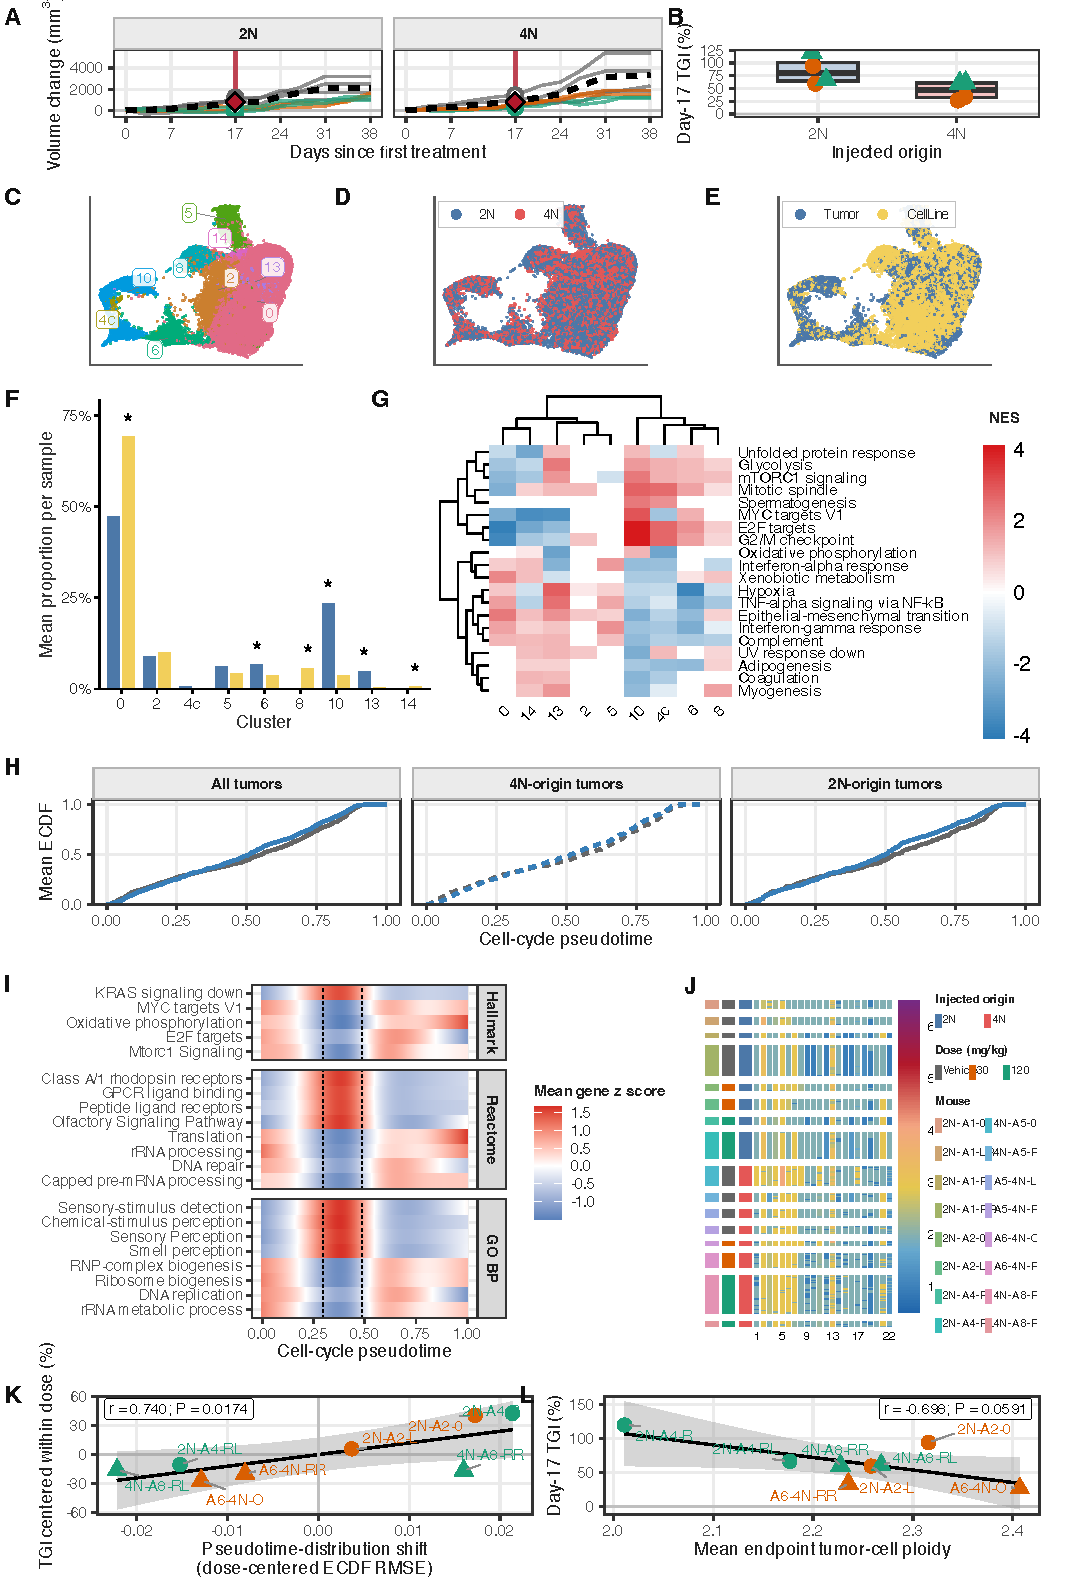
\includegraphics[width=7.1in]{figures/Figure7/Figure7_reviewed_GRCh.pdf}
\captionsetup{aboveskip=2pt,skip=0pt}
\caption{\scriptsize
\textbf{Tumor growth, tumor growth inhibition, cellular states, and endpoint ploidy in gemcitabine-treated SUM-159 xenografts.}
}
\label{fig:in_vivo_pseudotime_tgi}
\end{figure}

\begin{figure}[p]
\ContinuedFloat
\captionsetup{list=off}
\caption{\footnotesize
\textbf{Tumor growth, tumor growth inhibition, cellular states, and endpoint ploidy in gemcitabine-treated SUM-159 xenografts (continued; panels A--F).}
\textbf{(A)} Change in tumor volume from the first treatment day for 16 tumors initiated with near-diploid (2N) or near-tetraploid (4N) SUM-159 cells. Each injected-origin group comprised four vehicle-treated tumors and two tumors at each gemcitabine dose (30 and 120~mg/kg). Thin lines represent individual mice; gray, orange, and green denote vehicle, 30~mg/kg, and 120~mg/kg, respectively. Dashed black lines are the mean trajectories of vehicle-treated tumors matched by injected ploidy origin, and the vertical red line marks Day~17. Open circles mark individual-mouse Day-17 values; red diamonds mark the corresponding matched-control means. For each treated mouse, Day-17 tumor growth inhibition (TGI) was calculated as \(100\times[1-\Delta V_{\mathrm{treated}}/\overline{\Delta V}_{\mathrm{matched\ vehicle}}]\), where \(\Delta V\) is the change in tumor volume from Day~0.
\textbf{(B)} Day-17 TGI for the eight treated tumors, grouped by injected ploidy origin (\(n=4\) tumors per group). Blue and pink boxes denote 2N- and 4N-origin tumors, respectively; orange circles and green triangles denote 30 and 120~mg/kg, respectively. Boxes show the median and interquartile range; whiskers extend to the most extreme observation within 1.5 times the interquartile range, and all independent tumors are plotted. The dose-adjusted 4N-minus-2N difference was \(-39.5\) percentage points (exact permutation test stratified by dose, \(P=0.0556\)).
\textbf{(C)} Joint uniform manifold approximation and projection (UMAP) of 35,513 cells---9,832 final-QC tumor cells from 16 tumors and 25,681 cells from two cultured SUM-159 reference preparations---colored by the nine graph-based clusters; labels mark cluster locations.
\textbf{(D)} The same UMAP colored by injected tumor origin or cultured-reference ploidy, with blue indicating 2N and vermilion indicating 4N.
\textbf{(E)} The same UMAP colored by source context, with blue indicating xenograft tumor cells and yellow indicating cultured reference cells.
\textbf{(F)} Mean within-sample cluster proportions for the 16 tumors and two cultured reference samples. Cluster proportions were first calculated separately within each sample and then averaged with equal sample weight within each context; blue and yellow bars denote tumors and cultured references, respectively. Asterisks mark only positive enrichment of the indicated context for that cluster (\(*\), panel-wide Benjamini--Hochberg \(q\leq0.05\)), assessed by exact context-label permutation within 2N/4N strata.
}
\end{figure}

\begin{figure}[p]
\ContinuedFloat
\captionsetup{list=off}
\caption{\footnotesize
\textbf{Tumor growth, tumor growth inhibition, cellular states, and endpoint ploidy in gemcitabine-treated SUM-159 xenografts (continued; panels G--K).}
\textbf{(G)} Cluster-versus-rest Hallmark gene-set enrichment analysis for the nine-cluster landscape. The 20 gene sets with the largest maximum absolute normalized enrichment score (NES) across clusters are shown; rows and columns are hierarchically clustered independently. Red and blue indicate positive and negative NES, respectively. White cells displayed as zero are placeholders for cluster--pathway combinations lacking a finite NES; they do not denote nonsignificance, and this heatmap does not encode false-discovery rate.
\textbf{(H)} Equal-mouse mean empirical cumulative distribution functions (ECDFs) of cell-cycle-associated pseudotime for 2,881 tumor cells in clusters 4c, 6, and 10 across the 16 tumors (1,328 vehicle-treated and 1,553 gemcitabine-treated cells). Gray and blue curves denote vehicle and gemcitabine treatment, respectively. The combined comparison contains eight mice per group, and each injected-origin comparison contains four mice per group; solid curves show the combined and 2N-origin comparisons, whereas dashed curves show the 4N-origin comparison. The combined comparison gave RMSE \(=0.0378\) and exact mouse-label permutation \(P=0.00513\); the 4N- and 2N-origin comparisons gave RMSE \(=0.0317\), \(P=0.143\), and RMSE \(=0.0456\), \(P=0.0571\), respectively.
\textbf{(I)} Mouse-aware fitted pathway profiles across cell-cycle-associated pseudotime for the same 2,881-cell subset. Models included dose and injected ploidy origin; 14 mice contributed retained sample bins within the marked 0.30--0.49 interval. Dashed lines delimit this interval. Within each Hallmark, Reactome, or Gene Ontology Biological Process collection, up to four positively and four negatively enriched pathways were selected only when they passed collection-wide Benjamini--Hochberg \(q\leq0.05\); nonsignificant pathways were not substituted when fewer than four passed. For each pathway, the fitted trajectory of each leading-edge gene was standardized across pseudotime before the standardized gene trajectories were averaged. Red and blue therefore indicate relatively higher and lower mean standardized fitted expression, respectively. Enrichment direction compares the marked interval with its two neighboring pseudotime intervals and is not a direct treatment effect at fixed pseudotime.
\textbf{(J)} Association across the eight treated tumors between Day-17 TGI and ECDF displacement from the equal-mouse vehicle reference matched by injected ploidy origin; both variables were centered within dose. Each point is one mouse; text labels identify mice, orange and green indicate 30 and 120~mg/kg, and circles and triangles indicate 2N- and 4N-origin tumors, respectively. The black line is the linear fit and the gray band its 95\% confidence interval. The annotation reports Pearson's \(r\) and an exact within-dose permutation \(P\) value.
\textbf{(K)} Unadjusted association across the same eight treated tumors between Day-17 TGI and mean endpoint tumor-cell ploidy. NUMBAT-derived cell estimates were restricted to the 5,335 treated cells within the 9,832-cell final-QC tumor universe before calculating one mean per mouse. Text labels identify mice; point colors and shapes are as in J. The black line is the linear fit and the gray band its 95\% confidence interval. The annotation reports Pearson's \(r\) and an exact unrestricted permutation \(P\) value. Because the 2N- and 4N-origin cohorts were processed in separate NUMBAT runs with different segment schemas and calibration, this unadjusted association is descriptive and does not establish an origin- or dose-independent endpoint-ploidy effect. TGI, tumor growth inhibition; UMAP, uniform manifold approximation and projection; ECDF, empirical cumulative distribution function; RMSE, root-mean-square error; NES, normalized enrichment score.
}
\end{figure}
\endgroup
\clearpage


\section*{Discussion}



Our study identifies ploidy as a determinant of both the magnitude and kinetics of gemcitabine response. Across independent pharmacogenomic datasets, gemcitabine repeatedly emerged as a low-ploidy-selective cytotoxic agent, and this association was recapitulated across matched isogenic systems from multiple lineages. Our mechanistic analysis of near-diploid and near-tetraploid isogenic cell line pair further revealed that high-ploidy resistance was not explained by a failure to generate the active metabolite dFdCTP. Instead, 4N cells accumulated more dFdCTP while exhibiting weaker checkpoint activation, attenuated nucleotide-metabolic remodeling, reduced fitted cytostatic and cytotoxic potency, and a substantially longer delay before cell death. These findings support the SUM-159 live/dead model in which high ploidy alters the pharmacodynamic conversion of intracellular gemcitabine exposure to weaker replication stress, cytostatic transition and cytotoxic potency together with a substantially longer delay from effective intracellular dFdCTP exposure to observed cell death. Thus, the current data indicate a parsimonious interpretation in which ploidy reshapes gemcitabine response through altered effective drug-action mapping and delayed execution of cell death.

\begingroup
\renewcommand{\thefigure}{6}
\begin{wrapfigure}{r}{0.8\textwidth}
    \centering
    \vspace{-10pt}
\includegraphics[width=0.7\textwidth]{figures/Figure6_v6_Overleaf.png}
    \caption{\footnotesize \textbf{Ploidy state determines gemcitabine-induced metabolic remodeling and nucleotide depletion in SUM-159 cells.}
    (\textbf{A}) Principal component analysis (PCA) of untargeted metabolomics profiles from SUM-159 2N and 4N cells under control and gemcitabine-treated conditions. Each point represents an individual biological replicate. (\textbf{B}) Response category counts for metabolites with the predefined response threshold of 2-fold change and p < 0.05. Metabolites were classified as showing no strong response, 2N-specific response, 4N-specific response, common gemcitabine response or ploidy-specific differential response. (\textbf{C}) Curated pathway-class enrichment analysis of metabolite response categories. Enrichment was assessed using curated, name-based pathway classes. (\textbf{D}) Heatmap of metabolites with 2-fold or more change and p < 0.05 response threshold or showing ploidy-dependent differential response. Rows represent metabolites ordered by response class, and columns represent biological replicates from SUM-159 2N and 4N cells under control and gemcitabine-treated conditions. Values are shown as row-scaled z-scores. Changes in nucleotide-related metabolites are indicated with arrow heads. (\textbf{E}) Volcano plots showing metabolite-level responses to gemcitabine in SUM-159 2N cells, SUM-159 4N cells, and the ploidy-dependent differential response. For the 2N and 4N plots, the x-axis represents log2 fold change after gemcitabine treatment relative to control, and the y-axis represents $-\log_{10}(\text{p-value})$. For the differential-response plot, the x-axis represents $\Delta$log2 fold change, calculated as the 2N response minus the 4N response. Red points indicate metabolites passing p < 0.05 and $\ge$ 2-fold change. Core pyrimidine and purine metabolites are labeled to highlight nucleotide-associated changes.
    }
     \label{fig:metabolomics_response}
\end{wrapfigure}
\endgroup

The dissociation between dFdCTP accumulation and cytotoxic response is a central feature of our study. Canonical models of gemcitabine resistance frequently invoke reduced transport, impaired phosphorylation, enhanced inactivation or diminished intracellular retention. Our results indicate that active-metabolite abundance alone is insufficient to predict drug response across ploidy states. High-ploidy cells remained comparatively resistant despite accumulating substantial intracellular dFdCTP, suggesting that equivalent or even greater total metabolite exposure does not necessarily impose equivalent functional pressure on DNA synthesis. Ploidy may, therefore, influence gemcitabine response downstream of metabolic activation, through differences in the scale of nucleotide demand, the effective competition between dFdCTP and endogenous dCTP, the number and behavior of replication forks or the capacity to sustain DNA synthesis under nucleotide stress.

The checkpoint signaling provides a mechanistic anchor for the model-inferred ploidy-dependent potency shift. Gemcitabine induced stronger phosphorylation of CHK1, and to a lesser extent CHK2, at lower administered doses in 2N cells compared to 4N cells. Together with the intracellular PK/PD and live-cell measurements, this result indicates that lower-ploidy cells translate gemcitabine exposure into detectable replication-stress signaling more efficiently. However, checkpoint activation is not itself a direct measure of lethal damage because it can reflect both the magnitude of replication stress and the protective response mounted against it. Therefore, reduced checkpoint signal in 4N cells could arise from weaker initial nucleotide stress, delayed pathway engagement, enhanced replication-fork stabilization or altered tolerance of lesions that persist into mitosis.Future time-resolved and cell-cycle-resolved measurements will, thus, be needed to determine whether 4N cells experience less initial replication stress, delayed checkpoint activation, enhanced replication fork protection or greater tolerance of damage carried into mitosis.

The metabolomic data suggest that differential nucleotide homeostasis contributes to this phenotype. Gemcitabine produced broader metabolic remodeling in 2N cells, including stronger changes in pyrimidine- and purine-associated metabolites and a larger reduction in dCMP abundance whereas 4N cells showed a comparatively attenauted response. These findings suggest that gemcitabine sensitivity depends on the balance between demand, competing cytidine pools and nucleotide-buffering capacity. Proliferative 4N cells that have successfully adapted to genome doubling must support replication of an expanded DNA template and may consequently acquire increased nucleotide-production or salvage capacity to help buffer gemcitabine-induced cytidine-pathway perturbation. Therefore, such adaptations may incidentally reduce the effective replication-stress burden imposed by gemcitabine. In this framework, high-ploidy cells could be more resistant if they maintain a lower effective dFdCTP-to-dCTP pressure, either by accumulating larger competing cytidine pools, sustaining nucleotide replenishment, or reducing the functional impact of gemcitabine metabolites on DNA synthesis. This interpretation is also important for evaluating intracellular dFdCTP measurements: because 4N cells are larger, greater total dFdCTP accumulation in 4N cells (Fig. \ref{fig:dFdCTP_livedead}B), need not imply greater effective drug pressure per unit DNA, cell volume, replication fork, or competing cytidine nucleotide pool. However, because steady-state dCMP abundance does not directly measure dNTP pools or nucleotide flux, future isotope-tracing and targeted dNTP/dFdCTP measurements will be required to distinguish increased de novo synthesis from altered salvage, catabolism, nucleotide utilization or scaling effects related to cell size and DNA content.

A second, non-mutually exclusive interpretation is that higher-ploidy cells may also be better able to tolerate the chromosomal consequences of replication-stress-induced missegregation. Under-replicated DNA becomes most dangerous when cells enter mitosis before replication is complete, because unresolved loci can generate ultrafine anaphase bridges, chromatin bridges, acentric fragments, micronuclei and post-mitotic genome loss \cite{beeharry_centromere_2013,bhowmick_rad52_2016,kong_rif1_2023}. In this framework, high ploidy is not expected to be uniquely compatible with upstream pharmacologic resistance mechanisms, which primarily reduce effective intracellular drug burden. Instead, high ploidy is most compatible with downstream resistance mechanisms that require survival after imperfect genome duplication, including tolerance of under-replicated DNA entering mitosis, bridge or micronucleus resolution, senescence or PGCC-like persistence, and viable exit from abnormal mitoses \cite{song_gemcitabine_2016,ma_high-throughput_2025,kuznetsova_chromosomal_2015,quinton_whole-genome_2021}. Thus, our results suggest that gemcitabine resistance can arise not only by reducing the initial replication lesion, but also by increasing the probability that cells survive the chromosomal damage produced when replication stress is carried into mitosis.
  
Many anticancer drugs promote chromosome missegregation either directly, by disrupting mitosis, or indirectly, by generating replication and DNA-damage lesions that persist into mitosis. A ploidy-dependent survival framework predicts that near-diploid cells should be particularly vulnerable to CIN-inducing therapies, because missegregation events, especially chromosome-loss events, impose larger immediate fitness costs before genome doubling. Consistent with this prediction, previous pharmacogenomic analyses identified multiple mitotic spindle poisons, including paclitaxel, vinblastine, and vinorelbine, among the strongest ploidy-associated agents in breast cancers\cite{kimmel_integrating_2020}. Surprisingly, gemcitabine showed the strongest association with ploidy in this analysis. Although gemcitabine is classically viewed as an S-phase antimetabolite, an independent human artificial chromosome loss assay showed that it is also a potent inducer of chromosome loss, ranking among the highest CIN-inducing drugs tested and increasing chromosome loss by approximately 35--45-fold \cite{lee_effects_2016}. Independent drug-sensitivity studies have also identified gemcitabine as a low-ploidy-selective compound \cite{choudhary_identification_2016}. These observations nominate gemcitabine as an unexpected but compelling candidate for testing whether ploidy modifies chemotherapy response.

Our mathematical model formalizes this distinction between intracellular exposure and downstream effect. A model driven solely by the measured dFdCTP profiles was insufficient to reproduce the observed responses across doses and ploidy states. Incorporating a nonlinear dose transformation, ploidy-specific potency parameters and a distributed delay to death substantially improved the representation of the live and dead cell trajectories. The fitted model attributed the enhanced sensitivity of 2N cells to both stronger immediate cytostasis and greater delayed cytotoxicity, while estimating a more than twofold longer interval between effective drug action and observed death in 4N cells. These parameters should not be interpreted as direct measurements of individual molecular processes. Rather, they provide a quantitative summary of otherwise unresolved biological steps separating metabolite exposure from phenotypic outcome and identify the exposure-to-effect relationship—not drug accumulation alone—as the principal point of divergence between ploidy states. Moreover, this mathematical approach indicated that high-ploidy cells may translate intracellular gemcitabine exposure into a more attenuated metabolic response. Guided by this prediction of the model, metabolomic profiling revealed broader disruption of nucleotide-associated pathways in 2N cells than in 4N cells, providing a plausible metabolic basis for the stronger replication-stress response observed in the low-ploidy state. 

Altogether, our findings establish an experimental and mathematical framework in which ploidy functions as a quantitative cell-state variable governing gemcitabine response. High-ploidy cells do not simply accumulate less active drug; rather, they appear to buffer or delay the processes that connect dFdCTP exposure to nucleotide disruption, checkpoint activation, and cell death. This distinction has implications beyond gemcitabine. For therapies whose activity depends on DNA synthesis, genome copy number may determine both the effective burden imposed by treatment and the probability that damaged cells survive long enough to recover, persist, or re-enter the cell cycle. Incorporating ploidy into pharmacodynamic analyses may therefore reveal therapeutic dependencies that remain obscured when drug response is interpreted solely from extracellular dose or intracellular drug abundance.


\section{Methods}
% \subsubsection*{Model 1}

% Hypothesis 1: 
% Cells continue to divide under treatment, but most of them die in the process. Over time resistance develops as dividing cells reduce their apoptotic risk.\newline


% We use a log-kill pattern for modeling treatment effect, which assumes that the shrinkage rate of the population as a result of drug treatment is proportional to population size:


% \begin{equation} \label{m1}
% \frac{\mathrm{d} T}{\mathrm{~d} t}=f(T)-k_{\mathrm{d}} \cdot e^{-\lambda \cdot t} \cdot \text { Exposure } \cdot T
% \end{equation}

% The $e_{-\lambda \cdot t}$ term quantifies the decline of drug effect over time (i.e. resistance) and $f(T)$ is the growth term. For example, for logistic growth we have: $f(T) = r \cdot T \cdot (1 - \frac{T}{K})$


\subsection{Cell lines and isogenic ploidy validation}
  \label{sec:methods-cell-lines-ploidy-validation}

TNBC lines SUM-159 and MDA-MB-231 were a generous gift of Andriy Marusyk, and gastric cancer lines SNU-668 and HGC-27 were obtained from the ATCC. Cell-line identities were confirmed by
  short tandem repeat analysis of cellular DNA, and all cultures were routinely tested for Mycoplasma contamination. TNBC lines were cultured in McCoy medium (GIBCO, 16600), and gastric
  cancer lines were cultured in RPMI-1640 medium (GIBCO, 11875) supplemented with 10\% FBS (v/v; Gemini Bio, 900-108-500).

  Isogenic low- and high-ploidy cancer-cell pairs were generated by long-term density selection in SNU-668 \cite{veith_cloneid_2025} and by cell fusion \cite{su_somatic_2015} and long term hypoxia \cite{XX} in SUM-159.
  Additional matched low- and high-ploidy lineage pairs were included as indicated. For each isogenic pair, DNA-content differences were confirmed by flow cytometry and maintained for at
  least five passages before drug exposure.
  
\subsection{Reagents}
Gemcitabine (ChemieTek, CT-GEM) was purchased in powder form and stored at 10 or 20 mmol/L stock concentrations in DMSO at $-20^\circ$C. Phospho-CHK1 (Ser317; Cell Signaling Technology, rabbit mAb, 12302, 1:1,000 dilution), Phospho-CHK2 (Thr68; Cell Signaling Technology, rabbit mAb, 2661, 1:1,000 dilution), $\beta$-actin (MP Biomedicals, mouse mAb, 69100, 1:10,000 dilution) antibodies were used for immunoblotting assays. 

\subsection{Microplate drug-sensitivity assays} \label{sec:methods-microplate-drug-sensitivity}
SUM-159, MDA-MB-231, SNU-668 and HGC-27 cells (3,000 per well) were seeded in 96-well plates and incubated at $37^\circ$C for 24 hours. Treatments with vehicle (DMSO) or serial dilutions of the indicated compounds in 11 concentrations from 1 to 10,000 nmol/L were performed in triplicate (final DMSO concentration = 0.34\% in all wells). After 96 hours, media were removed and cell viability was measured with a CellTiter-Glo assay (Promega, G7573).
  
  For the Figure~\ref{fig:gem_convergent_evidence_iso}H dose-response/AUC analysis, sample-level responses were normalized to the corresponding
  untreated control mean. Four-parameter log-logistic dose-response curves were fit with \texttt{drc::LL.4}, and normalized AUC was calculated over a
  common log$_{10}$ dose interval from 0.005 to 0.9 $\mu$M. Mean sample ploidy was taken from CLONEID genome-perspective profiles when available;
  documented fallback ploidy values were used for legacy samples without a matched CLONEID profile.


\subsection{Crystal violet staining assay}
SUM-159 cells ($1 \times 10^5$ per well) were seeded in 12-well plates and incubated at $37^\circ$C for 24 hours. Treatments with vehicle (DMSO) or serial dilutions of the indicated compounds in 10 indicated concentrations were performed (final DMSO concentration = 0.34\% in all wells). After seven days, media were removed and cell growth was assessed with a crystal violet staining assay solution [6\% glutaraldehyde, 0.5\% crystal violet (w/v) in water].

\subsection{Western blotting}
In all, $2 \times 10^5$ cells were treated with the indicated compounds at indicated concentrations in 6-well format. Twenty-four hours after treatments, the culture medium was aspirated and cells were washed with PBS. Cells were lysed in RIPA lysis buffer (50 mmol/L Tris buffer pH 8, 150 mmol/L NaCl, 1\% NP-40, 0.5\% sodium, 0.1\% SDS, 0.5\% Sodium deoxycholate) supplemented with protease and phosphatase inhibitors. The protein concentrations of cell lysates were measured with the Protein DC assay (Bio-Rad, 500--0111). Phosphorylation of CHK1 and CHK2, and expression of $\beta$-actin (internal control) were monitored by immunoblotting with monoclonal antibodies. Protein band intensities were measured with the ImageQuant software and graphed, if indicated.

\subsection{Light microscope and immunofluorescence assay}
Cells in transparent bottom plates were used to monitor cell morphology and nuclear mCherry expression. Microscopic observations were performed on a Nikon or EVOS FL Cell Imaging System. Mean nuclear area of cells after the treatments with the indicated compounds were calculated with the ImageJ software and graphed. RGB images of cells were converted to CMYK, and visualized with monochromic magenta (red and blue) or cyan (green and blue) filters to reduce the endogenous autofluorescence and acquire a detailed view of the cellular structures of interest such as nucleus and centrosome, if indicated.


\subsection{Delay-aware pharmacodynamic (PD) model of gemcitabine response}
Let \(c\in\{2N,4N\}\) denote ploidy state and let \(\widetilde{C}_c(t,d)\) denote the fitted intracellular dFdCTP-like exposure signal for dose \(d\) (Supplementary Methods \ref{dFdCTPsignalsurface}). The delayed drug-effect signal is represented by the terminal compartment \(Z_{n,c}(t,d)\) of an \(n\)-stage transit chain driven by \(\widetilde{C}_c(t,d)\):
\begin{equation}
\label{eq:gem_prelim_activity_model}
\frac{dL_c}{dt}
=
\underbrace{
r_c
\frac{1}{1+k_{\mathrm{cyto},c}\widetilde{C}_c(t,d)}
L_c\left(1-\frac{L_c}{K_c}\right)
}_{\text{cytostasis-modulated growth}}
-
\underbrace{
\left[
\mu_{\mathrm{base},c}
+
\mu_{\mathrm{conf},c}\left(\frac{L_c}{K_c}\right)^q
+
k_{\mathrm{kill},c}A_{\mathrm{Gem},c}(t,d)
\right]L_c
}_{\text{baseline, confluence-associated, and gemcitabine-associated death}} .
\end{equation}
Here, \(L_c(t)\) denotes live-cell abundance, \(r_c\) is baseline growth rate, \(K_c\) is carrying capacity, \(k_{\mathrm{cyto},c}\) controls apparent cytostatic potency, \(\mu_{\mathrm{base},c}\) and \(\mu_{\mathrm{conf},c}\) capture baseline and confluence-associated death, and \(k_{\mathrm{kill},c}\) controls apparent cytotoxic potency. The transit-chain construction captures distributed delay from intracellular drug activity to observed death \cite{gross_analysis_2023,hurtado_building_2021}.


  
\subsection{Pharmacogenomic analysis of ploidy-associated drug classes} \label{sec:methods-gdsc-drug-classes}

  We integrated GDSC drug-response data \cite{yang_genomics_2013} with cell-line ploidy estimates from CellPassports \cite{vandermeer_cell_2018}. For each cancer type and drug, duplicate
  drug--cell-line records were resolved by retaining the measurement with the lowest finite RMSE, and we calculated the Pearson correlation between cell-line ploidy and the GDSC drug-
  response Z-score across matched cell lines. Drugs were assigned to 19 primary anticancer classes derived from Pubchem \cite{xx} and Drugbank; then grouped into 11 broader displayed categories. We then tested whether each drug category was enriched near the top of the signed ranked list using a one-sided rank-enrichment statistic analogous to a
  Kolmogorov--Smirnov running-sum statistic. Enrichment significance was estimated with 1000 random permutations of drug-category labels. Exact zero permutation \(p\)-values were replaced by
  the permutation floor \(1/(1000+1)\), and Benjamini--Hochberg FDR correction was applied across the displayed drug-category, cancer-context, and direction tests.
  Figure~\ref{fig:ploidy_drug_class_enrichment} reports enrichment at BH-FDR \(q \leq 0.05\)



\subsubsection{CCLE ploidy-associated drug sensitivity analysis}  \label{sec:methods-ccle}
  To locally reproduce the breast cancer CCLE ploidy--drug-response analysis, we matched breast cancer cell-line ploidy estimates to the legacy BreastCancerDrugSensitivity drug-response
  tables used by the original local analysis. These tables report drug-response \(Z\)-scores \cite{barretina_cancer_2012,ghandi_next-
  generation_2019,kimmel_integrating_2020}. Replicate or repeated drug entries within a cell line were averaged, and drugs were retained if they were observed in at least 80\% of the
  maximum drug coverage across matched cell lines. We then computed the Pearson correlation between cell-line ploidy and drug-response \(Z\)-score across matched cell lines. Lower
  \(Z\)-score values were treated as indicating greater drug sensitivity; therefore, positive correlations indicate that higher-ploidy lines tend to have higher \(Z\)-scores, consistent
  with relatively greater sensitivity in lower-ploidy lines. For visualization, retained drugs with \(|r| \geq 0.2\) were plotted.




\subsection{Cell viability and cell death assay}   \label{sec:methods-live-dead-assay}
Cell viability assays were carried out using the IncuCyte live-cell imaging system (Sartorius). Briefly, 2N and 4N SUM-159-NLS-mCherry cells were plated in four replicates in 96-well plates (Falcon, Corning, New York, USA) at a density of 2000 cells per well and treated with a 10-point 2X serial dilutions of gemcitabine within the concentration range of 0 and 800 nM. Sytox Deep Red (S11381, ThermoFisher Scientific) nucleic acid stain was also added to monitor dead cells. Plates were then incubated in the IncuCyte CO2 incubator for 10 days while four separate images were captured from each well every 2 hours using 10× objective in red, infrared and phase channels. Red object count (ROC) per well was calculated as a measure of viable cells and near-infrared object counts (NOC) per well was calculated as a measure of dead cells when the treatment was performed.
\subsection{Quantification of Gemcitabine Metabolites by LC–MS/MS}

SUM-159 cells were seeded and treated with vehicle or gemcitabine for the indicated time points up to 48 h. For each condition, $2 \times 10^{6}$ cells were collected, pelleted by centrifugation at 1,000 rpm for 5 min at $4^\circ$C, washed with cold PBS, flash frozen in liquid nitrogen, and stored at $-80^\circ$C until metabolite extraction. For extraction, frozen cell pellets were resuspended in 500 $\mu$L ice-cold methanol and vortexed vigorously. Samples were vortexed again and centrifuged at $16,000 \times g$ for 5 min at $4^\circ$C. A total of 700 $\mu$L supernatant was transferred to a new 1.5-mL tube and evaporated to dryness at $37^\circ$C using a centrifugal evaporator.

Dried extracts were reconstituted in 100 $\mu$L of 10 mmol/L ammonium bicarbonate/acetonitrile [35:65, v/v]. After centrifugation at $16,000 \times g$ for 5 min, 70 $\mu$L of the supernatant was transferred to LC-MS vials for analysis. Quantification of gemcitabine (dFdC), gemcitabine monophosphate (dFdCMP), gemcitabine diphosphate (dFdCDP), gemcitabine triphosphate (dFdCTP), and the deaminated metabolite 2',2'-difluorodeoxyuridine (dFdU) was performed using a Xevo TQ-S micro triple quadrupole mass spectrometer coupled to an ACQUITY UPLC H-Class Bio system (Waters).

Two microliters of each sample were injected onto a SeQuant ZIC-pHILIC column (5 μm, 4.6 × 150 mm; Merck Millipore) maintained under hydrophilic interaction chromatography conditions. The flow rate was 0.5 mL/min. Mobile phase A consisted of 10 mmol/L ammonium bicarbonate with 0.05\% ammonium hydroxide, and mobile phase B consisted of acetonitrile. The gradient was as follows: 0–5 min, linear gradient from 65\% B to 40\% B; 5–7 min, linear gradient to 0\% B; 7–9 min, isocratic at 0\% B; 9–9.1 min, linear gradient to 65\% B; and 9.1–15 min, isocratic at 65\% B for column re-equilibration.

Analytes were detected by multiple reaction monitoring in positive-ion mode using nitrogen as the nebulizing and desolvation gas and argon as the collision gas. Source conditions were as follows: ion source temperature, 150°C; desolvation temperature, 550°C; desolvation gas flow, 1,200 L/h; cone gas flow, 110 L/h; and capillary voltage, 2.0 kV. Representative MRM transitions were monitored using compound-specific cone voltages and collision energies optimized with authentic standards: dFdC, 264.1 > 112.0 (20 V, 15 eV); dFdCMP, 344.0 > 112.0 (20 V, 20 eV); dFdCDP, 424.0 > 112.0 (20 V, 25 eV); dFdCTP, 503.1 > 112.0 (20 V, 35 eV); and dFdU, 265.1 > 113.0 (20 V, 15 eV). 

Metabolite abundance was quantified by calculating the peak area ratio of each analyte to its corresponding internal standard. Calibration curves were generated using authentic metabolite standards spiked with matched internal standards and processed in parallel with experimental samples. Metabolite levels were normalized to cell number, and dFdCTP accumulation and dFdU formation were reported relative to time-zero controls, as indicated.

\subsection{PKPD measurement of intracellular dFdCTP}   \label{sec:methods-pkpd-dfdctp}
To construct the intracellular drug-action input for the live/dead model, we used PKPD measurements of gemcitabine metabolites collected for the matched 2N and 4N cell states. The live/dead model was driven by the intracellular active metabolite dFdCTP, rather than by parent gemcitabine concentration. For each ploidy, PKPD sheets corresponding to the main-dose and low-initial-dose gemcitabine conditions were used to define calibrated dFdCTP time courses. The main 2N and 4N PKPD sheets were treated as \(1.0~\mu\mathrm{M}\) gemcitabine reference-dose profiles, whereas the low-initial-gemcitabine 2N and 4N sheets were treated as \(0.1~\mu\mathrm{M}\) reference-dose profiles.

PKPD dFdCTP measurements were reported in ng/mL and converted to \(\mu\mathrm{M}\)-equivalent concentrations using the dFdCTP molecular weight,
\[
503.1~\mathrm{ng}/\mathrm{nmol}.
\]
Because
\[
1~\mathrm{nmol}/\mathrm{mL}=1~\mu\mathrm{M},
\]
the conversion was
\[
C_{\mathrm{dFdCTP}}~(\mu\mathrm{M})
=
\frac{C_{\mathrm{dFdCTP}}~(\mathrm{ng}/\mathrm{mL})}
{503.1~\mathrm{ng}/\mathrm{nmol}}.
\]
The resulting dFdCTP profiles were baseline-subtracted using the first measured time point so that the model input represented treatment-induced intracellular dFdCTP above the initial measured level.

\subsection{Image analysis}
 \subsubsection{Cell segmentation and classification with HALO}

Cell segmentation was achieved by training a single-cell segmentation neural network in Halo-AI platform \cite{indica_labs_halo_2023}. At the beginning, a training dataset was collected by selecting a subsample of images from the data. Two main selection criteria were considered during the image sampling. First, the training set must have representative images from both 2N and 4N cells. Second, multiple images were sampled from different time points for each cell type 2N and 4N to ensure the capture of cell change over time during the training process. After the selection of train set, nucleus of cells was labeled using Halo built-in labeling tools. Finally, the training process was performed until all cells are accurately segmented. 
Another object classifier was trained on the top of the cell segmentation classifier results to classify each segmented cell to either dead, alive or transitional cell. At the beginning, cells are labeled either dead or alive by tracking the cells over the time and by observing changes in their nuclei. The object classifier was trained iteratively until the cell were classified correctly.

\subsection{Western blotting}

Cells were seeded in 6-well plates at 2 × 10\^5 cells per well and treated with the indicated compounds at the indicated concentrations. Forty-eight hours after treatment, culture medium was aspirated and cells were washed once with cold PBS. Cells were lysed in ice-cold RIPA buffer containing 50 mmol/L Tris-HCl pH 8.0, 150 mmol/L NaCl, 1\% NP-40, 0.1\% SDS, and 0.5\% sodium deoxycholate, supplemented with protease and phosphatase inhibitor cocktails. Lysates were clarified by centrifugation at 14,000 × g for 10–15 min at 4°C, and protein concentrations were determined using the DC Protein Assay (Bio-Rad, 500-0111).

Equal amounts of protein were resolved by SDS-PAGE and transferred to low-fluorescence nitrocellulose membranes. Membranes were blocked in LI-COR Intercept Blocking Buffer for 1 h at room temperature and incubated overnight at 4°C with primary antibodies against phospho-CHK1, phospho-CHK2, and β-actin as an internal loading control. After washing with PBS-T, membranes were incubated for 1 h at room temperature with species-appropriate IRDye 680RD- or IRDye 800CW-conjugated secondary antibodies protected from light. Membranes were washed again with PBS-T followed by PBS and imaged using a LI-COR Odyssey infrared imaging system.

\subsection{Untargeted Metabolomics} \label{sec:methods-metabolomics}
Untargeted global metabolomics was performed on samples from SUM-159 cells via ultra-high performance liquid chromatography/tandem mass spectroscopy methods, including: 1) acidic positive ion conditions, one chromatographically optimized for more hydrophilic compounds, the other chromatographically optimized for more hydrophobic compounds; 2) basic negative ion optimized conditions; and 3) negative ionization. In total 474 compounds were detected in the samples. Raw signals were median normalized and missing values were imputed using the half minimum detected value for that compound.

Metabolite responses were tested by comparing gemcitabine-treated and control samples within each ploidy state using Welch's t-test on log2-transformed abundances. Features were
  classified as strong responses when \(|\log_2\mathrm{FC}| \geq 1\) and \(p < 0.05\). Ploidy-dependent differential responses were defined by a two-way ANOVA ploidy-by-treatment
  interaction with \(p < 0.05\) and \(|\Delta\log_2\mathrm{FC}_{2N-4N}| \geq 1\). The response heatmap (Fig. \ref{fig:metabolomics_response}B,C), displays the selected metabolites as row-wise z-scores across all individual samples.

\section*{Acknowledgements}
This work has been supported in part by the Flow Cytometry Core Facility at the Moffitt Cancer Center, an NCI designated Comprehensive Cancer Center (P30-CA076292).

\section*{Funding}
This work was supported by the NCI grants 1R03CA259873-01A1, 1R37CA266727-01A1 and 1R21CA269415-01A1 awarded to N. Andor. The funders had no role in study design, data collection and analysis, decision to publish, or preparation of the manuscript.


% \textcolor{blue}{\section*{Data and code availability} XX}

\clearpage

\section{Supplementary Information}


\renewcommand{\figurename}{Supplementary Figure}
\setcounter{figure}{0}  
\renewcommand{\tablename}{Supplementary Table}
\setcounter{table}{0}  

    
\subsection{In-vitro Delay-aware cytostasis and cytotoxicity model for gemcitabine} \label{LCTmodelinvitro}


\subsubsection{Intracellular dFdCTP signal surface.}\label{dFdCTPsignalsurface}
The default in vitro gemcitabine live/dead model is driven directly by a ploidy-specific intracellular dFdCTP signal surface rather than by parent extracellular gemcitabine pharmacokinetics. For ploidy $p\in\{2N,4N\}$, administered gemcitabine dose $d$ (in $\mu$M), and time $t$ (in days), the PK-derived intracellular signal is denoted
\[
C_{\mathrm{dFdCTP},p}^{\mathrm{PK}}(t,d).
\]
This signal surface is built from the \texttt{dFdCTP (ng/mL)} PKPD measurements after conversion to $\mu$M-equivalent units and subtraction of the baseline ($t=0$) signal for each calibrated PK sheet. Each calibrated dose retained its own measured time course. Terminal behavior was represented by a fitted exponential tail when the post-peak decay phase was identifiable; otherwise, a predefined fallback half-life of 1 day was used for that dFdCTP profile. Within the calibrated dose range, the surface interpolates dFdCTP values across dose in log-dose space. Below the minimum calibrated PK dose, the temporal profile at the minimum calibrated dose is preserved and scaled proportionally with dose. At zero administered dose, the intracellular dFdCTP signal is defined to be zero.
Above the maximum calibrated PK dose, the default implementation uses explicit linear extrapolation in log-dose space based on the calibrated dose profiles evaluated at time $t$.

\subsubsection{Effective dose-response correction.}
For the default fits reported here, we used the beta--Hill baseline/confluence-death model. The effective intracellular dFdCTP signal combines a ploidy-specific power-law dose correction with a shared normalized Hill dose gate,
\[
\widetilde{C}_{p}(t,d)
=
C_{\mathrm{dFdCTP},p}^{\mathrm{PK}}(t,d)
\left(\frac{d}{d_{\mathrm{ref},p}}\right)^{\beta_p-1}
G(d;EC_{50},h,d_{\mathrm{ref},p}),
\]
where $d_{\mathrm{ref},p}$ is the minimum calibrated PK reference dose for ploidy $p$ and $\beta_p$ is a ploidy-specific dose-scaling exponent. This choice preserves the PK-derived signal when $\beta_p=1$ and allows sublinear or supralinear effective dose scaling when $\beta_p\neq 1$. The shared Hill gate is
\begin{equation}
\label{dose-responsecorrection}
G(d;EC_{50},h,d_{\mathrm{ref},p})
=
\frac{H(d;EC_{50},h)}{H(d_{\mathrm{ref},p};EC_{50},h)},
\qquad
H(d;EC_{50},h)=\frac{d^h}{EC_{50}^h+d^h},
\end{equation}
where $EC_{50}$ and $h$ are shared fit parameters. At $d=0$, the effective signal is set to $\widetilde{C}_p(t,0)=0$.

\subsubsection{Immediate cytostasis and distributed delay to death.}
Drug-induced proliferation suppression is driven by the \emph{immediate} effective dFdCTP signal. The cytostatic multiplier is
\[
m_{\mathrm{cyto},p}(t,d)
=
\frac{1}{1+k_{\mathrm{cyto},p}\widetilde{C}_{p}(t,d)},
\]
where $k_{\mathrm{cyto},p}$ is a ploidy-specific cytostatic potency parameter and $m_{\mathrm{cyto},p}\in(0,1]$.

Drug-induced death is delayed through a linear transit chain of length $n$:
\[
\frac{dZ_{1,p}}{dt}
=
k_{\mathrm{tr},p}\left(\widetilde{C}_{p}(t,d)-Z_{1,p}\right),
\]
\[
\frac{dZ_{i,p}}{dt}
=
k_{\mathrm{tr},p}\left(Z_{i-1,p}-Z_{i,p}\right),
\qquad i=2,\ldots,n.
\]
Here $k_{\mathrm{tr},p}$ is a ploidy-specific transit rate and $Z_{n,p}(t)$ is the delayed effective signal used for death. This linear chain provides a gamma-like distributed delay from intracellular dFdCTP exposure to death commitment. The number of transit compartments $n$ is treated as a structural choice and selected by comparing fits over a small grid of integer candidate values, rather than estimated as a continuous parameter. For each replicate trajectory, the transit-chain states are initialized at zero, $Z_{i,p,r,d}(0)=0$ for $i=1,\ldots,n$. In the default analysis, the candidate grid was $n\in\{2,3,4,5,6,7\}$.

\subsubsection{Alive/dead cell-count dynamics.}
Let $A_p(t)$ denote the live-cell compartment and $D_p(t)$ the observed dead-cell compartment for ploidy $p$. The default model includes a ploidy-specific baseline death hazard $\mu_{\mathrm{base},p}$ and a ploidy-specific drug-induced death term
\[
\kappa_{\mathrm{Gem},p}(t,d)=k_{\mathrm{kill},p}Z_{n,p}(t),
\]
where $k_{\mathrm{kill},p}$ is the cytotoxic potency per unit delayed effective signal. Following the manuscript convention,
\[
\Phi_{\mathrm{Gem},p}(t,d)=\kappa_{\mathrm{Gem},p}(t,d).
\]
The default model also includes confluence-associated death through
\[
\mu_{\mathrm{ctrl},p}(A_p)
=
\mu_{\mathrm{base},p}
+
\mu_{\mathrm{conf},p}\left(\frac{A_p}{K_p}\right)^q,
\]
with fixed exponent $q=4$. The total death hazard is therefore
\[
\lambda_p(t,d)=\mu_{\mathrm{ctrl},p}(A_p(t))+\kappa_{\mathrm{Gem},p}(t,d).
\]
The corresponding live/dead dynamics are
\[
\frac{dA_p}{dt}
=
r_p\,m_{\mathrm{cyto},p}(t,d)\,
A_p\left(1-\frac{A_p}{K_p}\right)
-\lambda_p(t,d)A_p,
\]
\[
\frac{dD_p}{dt}
=
\lambda_p(t,d)A_p-k_{\mathrm{clear},p}D_p.
\]
Here $r_p$ is the ploidy-specific maximum proliferation rate, $K_p$ is the ploidy-specific carrying capacity, and $k_{\mathrm{clear},p}$ is the ploidy-specific disappearance or clearance rate of observed dead objects. 

\subsubsection{Replicate-specific initial conditions.}
Each well/replicate trajectory was initialized from its own first paired alive/dead observation. Specifically, for replicate \(r\), ploidy \(p\), and dose \(d\), the model initial conditions were set to
\[
A_{p,r,d}(0)=A_{\mathrm{obs},p,r,d}(t_0),
\qquad
D_{p,r,d}(0)=D_{\mathrm{obs},p,r,d}(t_0),
\]
where \(t_0\) denotes the first retained imaging time point. Thus, replicate-to-replicate differences in seeding density and initial dead-object count were carried forward directly through the trajectory-specific initial conditions. Only time points with paired finite alive and dead observations were retained for likelihood evaluation.


\subsubsection{Ploidy-specific partial pooling and calibration.}
The primary fit uses penalized maximum a posteriori partial pooling across ploidies in log-parameter space. For each positive ploidy-specific parameter $\alpha_p$,
\[
\log \alpha_p=\mu_{\alpha}+\delta_{\alpha,p},
\]
where $\mu_{\alpha}$ is a shared population-level log parameter and $\delta_{\alpha,p}$ is a ploidy-specific deviation penalized by a zero-centered Gaussian prior. In the default model, the ploidy-specific fitted parameters are
\[
r_p,\; K_p,\; k_{\mathrm{tr},p},\; k_{\mathrm{kill},p},\; k_{\mathrm{clear},p},\; k_{\mathrm{cyto},p},\; \beta_p,\; \mu_{\mathrm{base},p},\; \mu_{\mathrm{conf},p}.
\]
The default model also fits the shared Hill-gate parameters $(EC_{50},h)$. Simpler nested configurations, obtained by fixing $\beta_p$, disabling the Hill gate, or disabling confluence-associated death, were retained for sensitivity analyses.
The corresponding prior penalty added to the objective is
\[
\mathcal{P}_{\mathrm{prior}}
=
\frac{1}{2}\sum_{\alpha}\sum_{p}
\left(\frac{\delta_{\alpha,p}}{\sigma_{\alpha}}\right)^2,
\]
with prior standard deviations
$\sigma_r=\sigma_K=\sigma_{EC_{50}}=\sigma_h=0.75$,
$\sigma_{k_{\mathrm{tr}}}=\sigma_{k_{\mathrm{kill}}}=\sigma_{k_{\mathrm{clear}}}=\sigma_{k_{\mathrm{cyto}}}=\sigma_{\mu_{\mathrm{base}}}=\sigma_{\mu_{\mathrm{conf}}}=1.00$,
and $\sigma_{\beta}=0.50$.


\subsubsection{Optimization routine}

For model calibration, the alive-cell channel included only objects classified as Alive, whereas the dead-cell channel included objects classified as either Dead or Transitional. The calibration data consist of time-resolved live and dead object counts from IncuCyte assays across gemcitabine doses, replicates, and ploidies. Time is measured in days and administered gemcitabine dose in $\mu$M. The primary objective is a negative-binomial count likelihood evaluated on both the alive and dead channels. For an observed count $y$ with model mean $\mu$ and dispersion $\theta$,
\[
Y\sim\mathrm{NB}(\mu,\theta),
\qquad
\mathrm{Var}(Y)=\mu+\frac{\mu^2}{\theta}.
\]
Let $\theta_A$ and $\theta_D$ denote the dispersion parameters for alive and dead observations, respectively. The total objective minimized in the primary fit is
\[
\mathcal{L}
=
-\sum_{\mathrm{obs}}
\log p_{\mathrm{NB}}\!\left(A_{\mathrm{obs}}\mid A_{\mathrm{model}},\theta_A\right)
-\sum_{\mathrm{obs}}
\log p_{\mathrm{NB}}\!\left(D_{\mathrm{obs}}\mid D_{\mathrm{model}},\theta_D\right)
+\mathcal{P}_{\mathrm{prior}},
\]
where $\mathcal{P}_{\mathrm{prior}}$ is the Gaussian penalty associated with the ploidy-deviation terms in log space. Positive parameters are optimized on the log scale. Candidate transit-chain lengths $n$ are compared over a fixed integer grid, and the selected model is the one with the lowest raw posterior objective (data negative log-likelihood plus prior penalty). Optimization is performed with L-BFGS-B on an internally normalized objective for numerical conditioning, while raw negative log-likelihood and posterior objective values are retained for reporting and model comparison. ODE trajectories are solved with LSODA through \texttt{solve\_ivp}.
In the default configuration, the fitted positive parameters therefore comprise the ploidy-specific growth, delay, kill, clearance, cytostasis, dose-scaling, baseline-death, and confluence-death parameters together with the shared Hill-gate parameters $EC_{50}$ and $h$.

For calibration, live and dead counts were assembled into replicate-specific trajectories by matching observations across time, ploidy, gemcitabine dose, and well identity. The default analysis used the first 5 days of imaging data. Each trajectory was initialized from its own first paired alive/dead observation, and non-finite or unpaired alive/dead time points were excluded before likelihood evaluation. In the default phenotype aggregation, Alive objects defined the live channel, whereas Dead and Transitional objects together defined the dead channel.

\clearpage
\color{blue}
\subsubsection{Using the in vitro delay kernel to constrain the in vivo ploidy-structured model}

The in vitro gemcitabine live/dead model was used to estimate the delay distribution linking effective intracellular gemcitabine activity to observed cell death. We treated this temporal component as the most transferable part of the in vitro fit. Specifically, for ploidy class \(p\), the transit chain
\begin{align}
\frac{dZ_{1,p}}{dt}
&=
k_{\mathrm{tr},p}
\left(
\widetilde C_p(t)-Z_{1,p}
\right),\\
\frac{dZ_{i,p}}{dt}
&=
k_{\mathrm{tr},p}
\left(
Z_{i-1,p}-Z_{i,p}
\right),
\qquad i=2,\ldots,n_{\mathrm{tr}},
\end{align}
defines an empirical delay kernel from effective drug activity to death commitment. For a chain with \(n_{\mathrm{tr}}\) stages and rate \(k_{\mathrm{tr},p}\), the approximate mean delay is
\begin{equation}
\tau_p \approx \frac{n_{\mathrm{tr}}}{k_{\mathrm{tr},p}},
\end{equation}
with approximate variance
\begin{equation}
\mathrm{Var}(\tau_p) \approx \frac{n_{\mathrm{tr}}}{k_{\mathrm{tr},p}^2}.
\end{equation}

In downstream in vivo ploidy-structured models, we do not directly transfer the in vitro cytotoxic potency \(k_{\mathrm{kill},p}\) as a fixed in vivo killing rate. Instead, the in vitro estimates of \(n_{\mathrm{tr}}\), \(k_{\mathrm{tr},2N}\), and \(k_{\mathrm{tr},4N}\) define the delay distribution and its ploidy dependence. The absolute in vivo cytotoxic potency is calibrated to the in vivo tumor-burden and ploidy-composition data.




\subsection{Deoxycytidine rescues gemcitabine toxicity but does not explain ploidy-selective resistance}\label{supp:deoxycytidine}

To test whether exogenous pyrimidines could account for the ploidy-associated difference in gemcitabine sensitivity, we treated matched 2N and 4N SUM-159 cells with gemcitabine in the presence of candidate nucleotides and nucleosides. Deoxycytidine uniquely suppressed gemcitabine cytotoxicity in both ploidy states, consistent with prior reports that extracellular deoxycytidine can rescue cells from gemcitabine exposure \cite{https://pmc.ncbi.nlm.nih.gov/articles/PMC7357734}. Thus, deoxycytidine competition is a bona fide gemcitabine-resistance mechanism in SUM-159 cells. However, because rescue was observed in both 2N and 4N cells rather than selectively in the high-ploidy state, these data do not support exogenous deoxycytidine competition alone as the primary explanation for differential gemcitabine sensitivity between ploidy states.

Conditioned-media rescue was dominated by recipient ploidy: both 2N-CM and 4N-CM produced larger EC50 shifts in 4N recipients than in 2N recipients (26.9 vs. 16.25-fold for 2N-CM; 58.3 vs. 19.4-fold for 4N-CM). A donor-ploidy effect was also evident but context-dependent, with 4N-CM only modestly stronger than 2N-CM in 2N recipients (19.4 vs. 16.25-fold), yet more than two-fold stronger in 4N recipients (58.3 vs. 26.9-fold). The particularly strong effect of 4N-conditioned media on 4N recipient cells further suggests a donor--recipient interaction, in which 4N cells may both release more resistance-promoting deoxycytidine activity and respond more strongly to it.


  
\subsection{In-vivo Delay-aware cytostasis and cytotoxicity model for gemcitabine}
The in-vivo model applies the delay-aware live/dead ODE framework from the
in-vitro calibration directly to in-vivo tumor burden dynamics. The model maintains
three state variables for each tumour sample: the total alive (proliferating)
cell count $A(t)$, a five-stage transit chain
$\{Z_1(t),\ldots,Z_5(t)\}$ representing the distributed delay from
plasma drug exposure to lethal cell-fate commitment, and an observed dead
compartment $D(t)$.
The ODE system is:
\begin{align}
\frac{dA}{dt}
&=
r\,\frac{1}{1+k_{\mathrm{cyto}}\,C_{\mathrm{eff}}(t)}\,
A\!\left(1-\frac{A}{K}\right)
-
\left[
  \mu_{\mathrm{base}}
  +\mu_{\mathrm{conf}}\!\left(\frac{A}{K}\right)^{\!q}
  +k_{\mathrm{kill}}\,Z_{n_{\mathrm{tr}}}
\right]A,
\label{eq:invivo_dA}
\\
\frac{dZ_1}{dt}
&=
k_{\mathrm{tr}}\!\left(C_{\mathrm{eff}}(t)-Z_1\right),
\\
\frac{dZ_i}{dt}
&=
k_{\mathrm{tr}}\!\left(Z_{i-1}-Z_i\right),\qquad i=2,\ldots,n_{\mathrm{tr}},
\\
\frac{dD}{dt}
&=
\left[
  \mu_{\mathrm{base}}
  +\mu_{\mathrm{conf}}\!\left(\frac{A}{K}\right)^{\!q}
  +k_{\mathrm{kill}}\,Z_{n_{\mathrm{tr}}}
\right]A
-k_{\mathrm{clear}}\,D,
\label{eq:invivo_dD}
\end{align}
with fixed exponent $q=4$ and fixed chain length $n_{\mathrm{tr}}=5$
(carried from the in-vitro model selection).

\paragraph{Plasma PK drug signal.}
The effective drug signal is derived from plasma pharmacokinetics rather than
from measured intracellular dFdCTP.
For gemcitabine administered as a weekly IV bolus, the raw plasma concentration
at within-cycle time $t$ is
\[
C_{\mathrm{raw}}(t)
=
C_{\mathrm{peak}}\,
\exp\!\left(-\frac{\ln 2}{t_{1/2}}\,\bigl(t \bmod T_{\mathrm{period}}\bigr)\right),
\]
where $C_{\mathrm{peak}}$, $t_{1/2}$, and $T_{\mathrm{period}}$ are sample-level
PK parameters.
When the administered dose $d$ (mg$\,$kg$^{-1}$) is known,
$C_{\mathrm{peak}}$ is fixed via the intracellular PK/PD linear model
$C_{\mathrm{peak}}=0.00971\times d$.
The effective signal is then obtained by the same dose-scaling correction
as in the in-vitro model,
\[
C_{\mathrm{eff}}(t)
=
C_{\mathrm{raw}}(t)\,
\left(\frac{C_{\mathrm{peak}}}{C_{\mathrm{peak,ref}}}\right)^{\!\beta-1},
\]
where $C_{\mathrm{peak,ref}}=0.00971\times120~\mathrm{mg\,kg^{-1}}$ is the
reference peak concentration at the maximum clinical dose, and $\beta$
is a fitted dose-scaling exponent.
When no drug is applied, $C_{\mathrm{eff}}(t)\equiv 0$ and the ODE reduces to logistic growth with drug-independent death.

\paragraph{Ploidy-derived transit rate.}
The transit rate $k_{\mathrm{tr}}$ is not fitted; it is derived from the
tumor's initial ploidy composition using the log-linear interpolation
calibrated on the in-vitro 2N and 4N estimates
(Section~\ref{LCTmodelinvitro}):
\[
k_{\mathrm{tr}}
=
\frac{n_{\mathrm{tr}}}{\tau(\bar{p})},
\qquad
\log\tau(\bar{p})
=
b_0 + b_1\log\!\left(\frac{\bar{p}}{2}\right),
\]
where $\bar{p}$ is the weighted-mean ploidy ratio of the pre-treatment
ploidy distribution, $b_0=\log(n_{\mathrm{tr}}/k_{\mathrm{tr,2N}})$,
and
$b_1=\log\!\bigl[(n_{\mathrm{tr}}/k_{\mathrm{tr,4N}})/(n_{\mathrm{tr}}/k_{\mathrm{tr,2N}})\bigr]/\log 2$,
with $k_{\mathrm{tr,2N}}=6.84~\mathrm{day}^{-1}$ and
$k_{\mathrm{tr,4N}}=2.82~\mathrm{day}^{-1}$.

\paragraph{Initialisation.}
The simulation starts at the first treatment day ($t_0=t_{\mathrm{tx}}$).
The initial alive cell count $A(t_0)$ is the total count of alive cells from the pre-treatment oxygen supply--demand model.
The Transit-chain states are initialized to zero $Z_i(t_0)=0$.
The conversion factor per-sample cells-per-cm$^3$ is derived as the
ratio of this initial cell count to the tumor volume observed at $t_0$
and is applied throughout to convert caliper-measured volumes to cell counts.

\paragraph{Data stream.}
Serial caliper measurements of tumour volume (cm$^3$) collected at days
$\{d_1,d_2,\ldots\}$ on or after the first treatment are converted to
total cell counts using the per-sample density factor.
Only days with a positive observed volume are retained.
The karyotype (biopsy) likelihood is not used by this model because
chromosome-number distributions are not simulated.


\subsubsection{Likelihood and objective function}
\label{sec:invivo_likelihood}

Let $\{(d_i,V_i^{\mathrm{obs}})\}$ denote the observed tumor burden
timeline ($V_i^{\mathrm{obs}}$ in cell counts).

\paragraph{Burden likelihood.}
Observed and predicted total burden are assumed to be log-normally
distributed about each other:
\[
\mathcal{L}_B
=
\sum_{i}
\left[
  \log\sigma_B
  +\tfrac{1}{2}\log(2\pi)
  +\frac{\bigl(\log V_i^{\mathrm{obs}}-\log A(d_i)\bigr)^2}{2\sigma_B^2}
\right],
\]
where $A(d_i)$ is the ODE-predicted alive cell count at day $d_i$ and
$\sigma_B$ is a shared log-scale noise parameter.
If either $V_i^{\mathrm{obs}}\le 0$ or $A(d_i)\le 0$ the proposal is
rejected.

\paragraph{PK priors.}
Gemcitabine PK parameters that are free (half-life $t_{1/2}$, dosing
interval $T_{\mathrm{period}}$, and, when the dose is unknown, $C_{\mathrm{peak}}$)
are assigned independent log-normal priors
$\log\theta_k\sim\mathcal{N}(\log\theta_k^{\mathrm{init}},\sigma_k^2)$.
Each prior contributes a Gaussian penalty:
\[
\mathcal{P}_{\mathrm{PK}}
=
\frac{1}{2}\sum_k
\left(
\frac{\log\theta_k-\log\theta_k^{\mathrm{init}}}{\sigma_k}
\right)^{\!2}.
\]

\paragraph{Total objective.}
The quantity minimised is:
\[
\mathcal{L}=\mathcal{L}_B+\mathcal{P}_{\mathrm{PK}}.
\]


\subsubsection{Fitted and fixed parameters}
\label{sec:invivo_params}

\paragraph{Fitted parameters.}
All parameters are optimised on the log scale.
The free parameters are listed in Table~\ref{tab:invivo_params_new}.

\begin{table}[h!]
\centering
\caption{Fitted parameters of the in-vivo live/dead model.}
\label{tab:invivo_params_new}
\begin{tabular}{llll}
\hline
Parameter & Symbol & Log-scale bounds & Initial value \\
\hline
Max.\ proliferation rate (day$^{-1}$) & $r$ &
  $[\log 10^{-3},\,\log 5]$ & $1.25$ \\
Carrying capacity (cells) & $K$ &
  $[\log 10^{2},\,\log 10^{10}]$ & $25\,358$ \\
Cytotoxic potency & $k_{\mathrm{kill}}$ &
  $[\log 10^{-5},\,\log 10^{7}]$ & $217.3$ \\
Dead-cell clearance rate (day$^{-1}$) & $k_{\mathrm{clear}}$ &
  $[\log 10^{-4},\,\log 20]$ & $0.152$ \\
Cytostatic potency & $k_{\mathrm{cyto}}$ &
  $[\log 10^{-4},\,\log 10^{7}]$ & $8041$ \\
Dose-scaling exponent & $\beta$ &
  $[\log 0.05,\,\log 3]$ & $0.253$ \\
Baseline death hazard (day$^{-1}$) & $\mu_{\mathrm{base}}$ &
  $[\log 10^{-5},\,\log 2]$ & $0.117$ \\
Confluence death hazard (day$^{-1}$) & $\mu_{\mathrm{conf}}$ &
  $[\log 10^{-5},\,\log 2]$ & $0.051$ \\
Burden log-noise & $\sigma_B$ &
  $[\log 0.01,\,\log 5]$ & $0.5$ \\
Gemcitabine half-life (days) & $t_{1/2}$ & PK prior & $0.05$ \\
Gemcitabine dosing interval (days) & $T_{\mathrm{period}}$ & PK prior & $7.0$ \\
Gemcitabine $C_{\mathrm{peak}}$ (dose unknown only) & $C_{\mathrm{peak}}$ & PK prior & $0.032$ \\
\hline
\end{tabular}
\end{table}

Initial values for the nine biological parameters are taken from the 2N
in-vitro MAP estimates (Table~\ref{tab:gem_best_fit_parameters}) as a
warm start; the MCMC then moves them toward the in-vivo posterior.

\paragraph{Fixed parameters.}
The following quantities are held fixed during calibration:
transit-chain length $n_{\mathrm{tr}}=5$;
transit rate $k_{\mathrm{tr}}$ (derived from initial ploidy as described above);
confluence-death exponent $q=4$;
reference peak concentration $C_{\mathrm{peak,ref}}=0.00971\times120~\mathrm{mg\,kg^{-1}}$;
ODE integration step $\Delta t=0.05~\mathrm{days}$;
haploid reference $N_{\mathrm{haploid}}=23$.
When the administered dose $d$ is known,
$C_{\mathrm{peak}}=0.00971\times d$ is also fixed.


\subsubsection{Optimization routine}
\label{sec:invivo_optim}

Parameters are sampled by a random-walk Metropolis algorithm run on
$N_{\mathrm{chains}}=32$ parallel chains simultaneously.
All parameters are maintained in log space; proposals for chain $j$ at
iteration $t$ are
\[
\theta_j^{(t)}
=
\theta_j^{(t-1)}+\epsilon^{(t)},
\quad
\epsilon^{(t)}\sim\mathcal{N}\!\left(\mathbf{0},\mathrm{diag}(s^2)\right),
\]
where $s$ is the per-dimension step-size vector, and proposals outside the
hard bounds are rejected by clamping.
The acceptance criterion is the standard Metropolis rule: a proposal is
accepted if
$\log U < \mathcal{L}(\theta^{(t-1)})-\mathcal{L}(\theta^{(t)})$
for $U\sim\mathrm{Uniform}(0,1)$.

\paragraph{Adaptation.}
During the burn-in phase ($N_{\mathrm{burnin}}=600$ iterations), the
step-size vector is adapted every 50 iterations: if the mean
chain-averaged acceptance rate falls below $0.234-0.05$, steps are
shrunk by a factor of $0.8$; if it exceeds $0.234+0.05$ they are grown
by $1.2$.
The target acceptance rate of $0.234$ is the asymptotically optimal rate
for a random-walk Metropolis sampler in high dimensions.

\paragraph{Sampling.}
Following burn-in, $N_{\mathrm{samples}}=1400$ sampling iterations are
run.
Posterior samples are collected every 2 iterations from
all 32 chains, giving up to
$1400/2\times 32=22{,}400$ posterior draws.
The maximum-a-posteriori estimate is tracked as the parameter
vector with the lowest objective value seen across all chains and all
iterations.

\paragraph{Parallelisation.}
Each chain evaluation requires a full ODE forward pass through the
treatment schedule.
Chains are evaluated in parallel using a persistent worker pool
($\min(32,\,N_{\mathrm{cpu}})$ processes) to avoid the overhead of
repeated process spawning.
The burden timeline is extracted from a single ODE integration per chain
per iteration.

\subsubsection{Drug delay}

For chromosome state \(j\), with chromosome number \(N_j\), we write the delayed in vivo drug signal as
\begin{align}
\frac{dZ_{1,j}}{dt}
&=
k_{\mathrm{tr}}(N_j)
\left(
\widetilde C_{\mathrm{in vivo}}(t)-Z_{1,j}
\right),\\
\frac{dZ_{i,j}}{dt}
&=
k_{\mathrm{tr}}(N_j)
\left(
Z_{i-1,j}-Z_{i,j}
\right).
\end{align}
, with $n_{tr}$, $k_{tr}$ given in table \ref{bestfitparams}. The gemcitabine-induced death component is then
\begin{equation}
\kappa_{\mathrm{Gem},j}(t)
=
k_{\mathrm{kill}}(N_j) Z_{n,j}(t).
\end{equation}


When a continuous chromosome-number dependence is required, we use a low-dimensional interpolation for the delay scale rather than fitting an independent delay parameter for every chromosome state. For example,
\begin{equation}
\log \tau(N)
=
b_0
+
b_1\log\left(\frac{N}{N_{2N}}\right),
\end{equation}
with priors chosen so that \(\tau(N_{2N},0)\) and \(\tau(N_{4N},1)\) are centered on the in vitro estimates. Equivalently, \(k_{\mathrm{tr}}(N)=n_{\mathrm{tr}}/\tau(N)\).


\color{black}


\clearpage

  \begin{table}[htbp]
  \centering
  \caption{Best-fit parameters for the in-vitro gemcitabine live/dead model.}
  \label{tab:gem_best_fit_parameters}
  \begin{tabular}{llp{6.2cm}cc}
  \toprule
  Parameter & Units & Brief definition & 2N & 4N \\
  \midrule
  \(r\) & day\(^{-1}\) & Max. proliferation rate of live cells & 1.25 & 1.78 \\
  \(K\) & cells (or live objects) & Carrying capacity & 25,358 & 20,512 \\
  \color{blue}\(k_{\mathrm{tr}}\) & \color{blue}day\(^{-1}\) & \color{blue}Transit rate governing delay from effective dFdCTP exposure to death signal & \color{blue}6.84 & \color{blue}2.82 \\
  \color{blue}\(n_{\mathrm{tr}}\) & \color{blue}dimensionless & \color{blue}Number of transit compartments in the linear-chain delay model & \color{blue}5 & \color{blue}5 \\
  \(k_{\mathrm{kill}}\) & day\(^{-1}\)\((\mu\mathrm{M\ dFdCTP})^{-1}\) & Cytotoxic potency per unit delayed intracellular drug signal & 217.3 & 129.9 \\
  \(k_{\mathrm{clear}}\) & day\(^{-1}\) & Clearance/disappearance rate of observed dead cells & 0.152 & 0.062 \\
  \(k_{\mathrm{cyto}}\) & \((\mu\mathrm{M\ dFdCTP})^{-1}\) & Cytostatic potency controlling suppression of proliferation by intracellular drug  & 8041 & 1163 \\
  \(\beta\) & dimensionless & Dose-scaling exponent: administered gemcitabine -->  intracellular drug signal & 0.253 & 0.488 \\
  \(\mu_{\mathrm{base}}\) & day\(^{-1}\) & Baseline drug-independent death hazard & 0.117 & 0.017 \\
  \(\mu_{\mathrm{conf}}\) & day\(^{-1}\) & Confluence-associated death hazard scale & 0.051 & 0.054 \\
  \bottomrule
  \end{tabular}
  \end{table}

  
\clearpage

  \begin{table}[ht]
  \centering
  \footnotesize
  \caption{Symbol table.}
  \label{tab:ntr_model_comparison}
  \begin{tabular}{p{0.1\linewidth}p{0.23\linewidth}p{0.15\linewidth}p{0.25\linewidth}p{0.19\linewidth}}
  \hline
LaTeX symbol & Implementation name & Unit & Brief definition & Best-fit/default value \\
\hline
$A_p(t)$ & alive state & cell/object count & Live-cell count state for ploidy $p$. & Replicate-specific $A_{0,\mathrm{rep}}$; dynamic prediction. \\
$D_p(t)$ & dead state & cell/object count & Observed dead-cell count state for ploidy $p$. & Replicate-specific $D_{0,\mathrm{rep}}$; dynamic prediction. \\
$C_{\mathrm{dFdCTP},p}^{\mathrm{PK}}(t,d)$ & \texttt{DfdctpSignalSurface} & $\mu$M-equivalent dFdCTP & PK-derived intracellular dFdCTP signal before beta/Hill correction. & Derived from PKPD workbook; not a fitted scalar. \\
$\widetilde{C}_{p}(t,d)$ & effective corrected dFdCTP signal & $\mu$M-equivalent effective dFdCTP & Effective dFdCTP signal after beta correction and Hill gate. & Computed from $C_{\mathrm{dFdCTP},p}^{\mathrm{PK}}$, $\beta_p$, $EC_{50}$, and $h$. \\
$d_{\mathrm{ref},p}$ & \texttt{min\_calibration\_dose\_uM} & $\mu$M & Minimum calibrated PK reference dose for normalization. & 2N: 0.1; 4N: 0.1. \\
$\beta_p$ & \texttt{beta\_dose} & dimensionless & Ploidy-specific power-law dose-scaling exponent. & 2N: 0.2533; 4N: 0.4877. \\
$EC_{50}$ & \texttt{dose\_gate\_ec50\_uM} & $\mu$M & Shared Hill-gate half-activation dose. & 0.018529 $\mu$M (18.529 nM). \\
$h$ & \texttt{dose\_gate\_hill} & dimensionless & Shared Hill coefficient for dose gate. & 2.6928. \\
$Z_{i,p}$ & transit compartments & $\mu$M-equivalent effective dFdCTP & Transit-chain state $i$ for delayed drug-death signal. & Dynamic state; not separately fitted. \\
$n$ & \texttt{n\_tr} & compartment count & Number of transit compartments selected by model comparison. & 5. \\
$k_{\mathrm{tr},p}$ & \texttt{k\_tr} & day$^{-1}$ & Ploidy-specific transit-chain rate. & 2N: 6.8427; 4N: 2.8202. \\
$k_{\mathrm{cyto},p}$ & \texttt{k\_cyto} & ($\mu$M-equivalent dFdCTP)$^{-1}$ & Ploidy-specific cytostatic potency. & 2N: 8040.9143; 4N: 1163.1135. \\
$k_{\mathrm{kill},p}$ & \texttt{k\_kill} & day$^{-1}$($\mu$M-equivalent dFdCTP)$^{-1}$ & Ploidy-specific cytotoxic potency per delayed signal. & 2N: 217.2640; 4N: 129.8923. \\
$r_p$ & \texttt{r} & day$^{-1}$ & Ploidy-specific maximum proliferation rate. & 2N: 1.2464; 4N: 1.7809. \\
$K_p$ & \texttt{K} & cell/object count & Ploidy-specific carrying capacity. & 2N: 25,358.2284; 4N: 20,512.0674. \\
$k_{\mathrm{clear},p}$ & \texttt{k\_clear} & day$^{-1}$ & Ploidy-specific disappearance rate for observed dead objects. & 2N: 0.1518; 4N: 0.0616. \\
$\mu_{\mathrm{base},p}$ & \texttt{mu\_base\_death} & day$^{-1}$ & Ploidy-specific drug-independent baseline death hazard. & 2N: 0.1168; 4N: 0.0174. \\
$\mu_{\mathrm{conf},p}$ & \texttt{mu\_confluence\_death} & day$^{-1}$ & Confluence-associated death scale at $A_p/K_p=1$. & 2N: 0.0514; 4N: 0.0541. \\
$q$ & \texttt{confluence\_death\_exponent} & dimensionless & Fixed exponent for confluence-associated death. & 4.0. \\
$\theta_A$ & \texttt{theta\_alive} & count-dispersion parameter & Negative-binomial overdispersion for alive counts. & 6.9519. \\
$\theta_D$ & \texttt{theta\_dead} & count-dispersion parameter & Negative-binomial overdispersion for dead counts. & 7.7583. \\
  \hline
  \end{tabular}
  \end{table}



\color{blue}

\begin{table}[htbp!]
\centering
\caption{Combined effective dose-correction factors in the best-fit model. Values are normalized to the 100 nM reference dose.}
\label{tab:effective_dose_scaling}
\begin{tabular}{lcc}
\toprule
Gemcitabine dose & 2N correction & 4N correction \\
\midrule
3.125 nM & 0.111 & 0.049 \\
6.25 nM & 0.408 & 0.213 \\
12.5 nM & 1.229 & 0.755 \\
25 nM & 1.967 & 1.421 \\
50 nM & 1.586 & 1.348 \\
100 nM & 1.000 & 1.000 \\
200 nM & 0.601 & 0.707 \\
400 nM & 0.359 & 0.497 \\
800 nM & 0.214 & 0.348 \\
\bottomrule
\end{tabular}
\end{table}



% \subsection{Drug-independent death and confluence-associated death are required to explain untreated controls}

% The 0 nM control wells exhibited measurable dead-object accumulation, which cannot be generated by a purely drug-induced death term because the dFdCTP signal is zero at zero gemcitabine dose. The best model therefore included both low-density baseline death and confluence-associated death. The fitted low-density baseline death rate was higher in 2N cells than in 4N cells, with \(\mu_{\mathrm{base},2N}=0.117~\mathrm{day}^{-1}\) and \(\mu_{\mathrm{base},4N}=0.017~\mathrm{day}^{-1}\). In contrast, the confluence-associated death scale was similar between ploidies, with \(\mu_{\mathrm{conf},2N}=0.051~\mathrm{day}^{-1}\) and \(\mu_{\mathrm{conf},4N}=0.054~\mathrm{day}^{-1}\), using a fixed confluence exponent \(q=4\).

% Including confluence-associated death also yielded carrying capacities with the expected ploidy ordering. The fitted carrying capacity was \(K_{2N}=25{,}358\) alive objects and \(K_{4N}=20{,}512\) alive objects, consistent with 4N cells reaching effective confluence at a lower object count. This suggests that the density-dependent death term prevented \(K\) from absorbing late control-well death dynamics and improved the biological interpretability of the fitted growth parameters.


\clearpage[t!]
    \centering
\begin{figure}
\includegraphics{figures/Supp_Figure1_v3_Overleaf.png}
\caption{\textbf{Expanded landscape of ploidy-associated drug-class enrichment across cancer cell lines.}
(\textbf{A}) Heatmap showing drug classes enriched among compounds with response patterns consistent with preferential low-ploidy sensitivity. Rows indicate cancer types and columns indicate curated drug classes. Color represents enrichment significance as $-\log_{10}(p)$, with larger values indicating stronger enrichment. (\textbf{B}) Heatmap showing drug classes enriched among compounds with response patterns consistent with preferential high-ploidy sensitivity, using the same row order, column order, and color scale as in panel A. Stars indicate nominal enrichment significance at $p \leq 0.05$. Exact zero values from permutation testing were plotted at the empirical permutation floor to avoid infinite $-\log_{10}(p)$ values. (GDSC: Genomics of Drug Sensitivity in Cancer, AUC: Area Under Curve)}
\label{fig:supp_gdsc_ploidy_enrichment}
\end{figure}


\clearpage

 \begin{figure}
\includegraphics{figures/Supp_Figure1_Overleaf.png}
\caption{\textbf{The delay-aware model recapitulates dose-dependent live and dead cell dynamics in both ploidy states.}
  (A) Joint cohort-level fits for near-diploid (2N) and (B) near-tetraploid (4N) SUM-159 cells. In each dose panel, points show observed alive and
  dead cells counts as objects over time across replicate wells.  Solid and dashed curves show the
  corresponding model-predicted alive and dead trajectories from the best cohort-level fit.
  The fitted model was the intracellular dFdCTP-driven model, with immediate
  cytostasis, delayed drug-induced death, ploidy-specific $\beta$ dose correction, a fitted
  shared Hill dose gate, baseline death, and fitted confluence-associated death. Parameters
  were inferred jointly across doses within each ploidy using the alive/dead negative-binomial
  objective. Control ($0$ nM) trajectories are included to show baseline growth and death
  behavior in the absence of treatment.}
\label{fig:default_gem_live_dead_fit}
\end{figure}

\clearpage

\begin{figure}
\includegraphics{figures/Supp_Figure3_v2_Overleaf.png}
\caption{\textbf{Complementary gemcitabine dose-response metrics support a directional association between increasing  ploidy and gemcitabine resistance.}
  (\textbf{A}) Relationship between mean cell ploidy and fitted gemcitabine EC50 across individual samples.
  (\textbf{B}) Relationship between mean cell ploidy and fitted gemcitabine IC50 across samples for which IC50 could be estimated.
  (\textbf{C}) Paired comparison of the change in normalized gemcitabine dose-response AUC versus the change in mean ploidy between low- and high-ploidy isogenic lineage-
  pairs.
  Across these complementary metrics, higher ploidy showed directionally positive associations with reduced gemcitabine sensitivity, although the EC50, IC50, and paired
  delta-AUC associations did not reach statistical significance.
}
\label{fig:gemcitabine_ploidy_response}
\end{figure}

\clearpage

\begin{figure}[p]
\centering
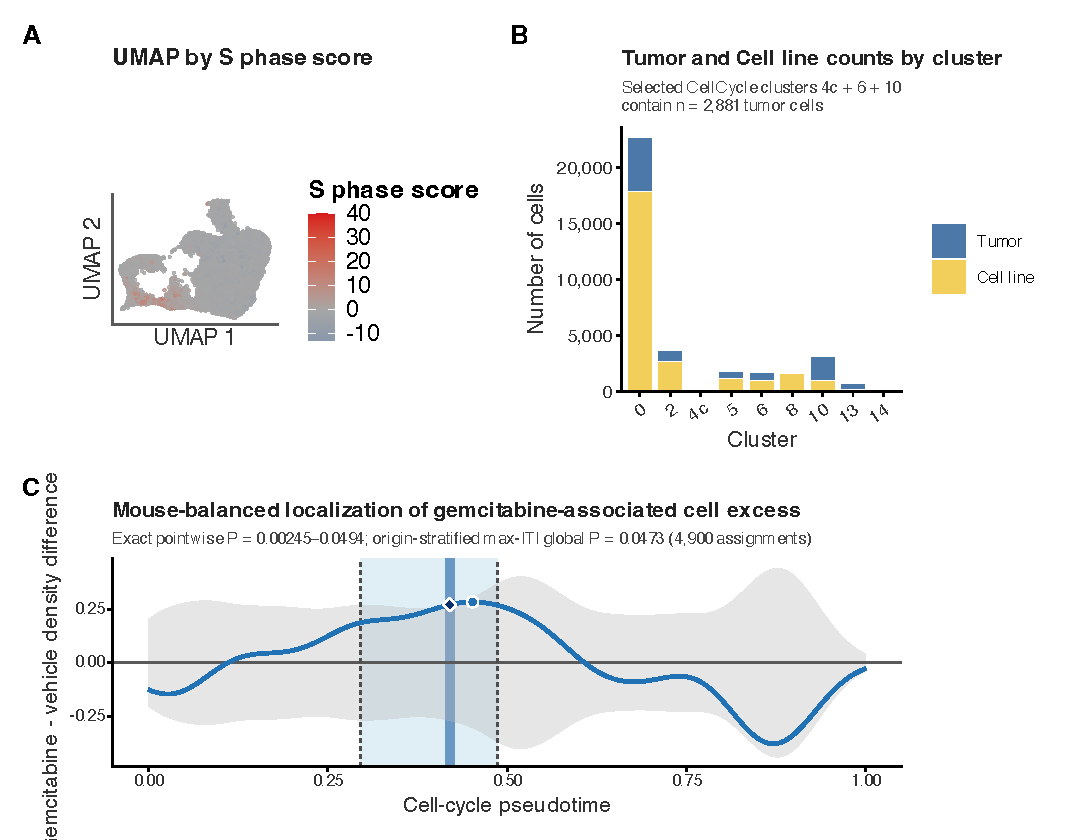
\includegraphics[width=\textwidth,height=0.88\textheight,keepaspectratio]{figures/Supplementary/panel_SuppFig4_composite.pdf}
\caption{\footnotesize
\textbf{Integrated tumor and CellLine cellular landscape.}
\textbf{(A)} Joint UMAP colored by the nine graph-based clusters.
\textbf{(B)} Joint UMAP colored by initial 2N or 4N ploidy.
\textbf{(C)} Joint UMAP distinguishing xenograft-derived tumor cells from cultured CellLine reference cells.
\textbf{(D)} Joint UMAP colored by S-phase score.
\textbf{(E)} Mean within-sample cluster proportions for the Tumor and CellLine contexts; every sample contributes equally within its context, and asterisks mark positive context enrichment at panel-wide BH FDR $\leq 0.05$ using exact sample-label permutations within initial-ploidy strata.
\textbf{(F)} Raw Tumor and CellLine cell counts by cluster; the subtitle identifies clusters 4c, 6, and 10 as the selected CellCycle subset and reports their summed 2,881 xenograft-derived cells.
\textbf{(G)} Mean within-sample cluster proportions by initial ploidy, with equal sample weights; asterisks mark positive ploidy enrichment using exact permutations within Tumor/CellLine context and the same panel-wide BH convention as in E.
\textbf{(H)} Raw cell counts by cluster and initial ploidy.
}
\label{fig:supp_cellular_landscape}
\end{figure}

\clearpage

\begin{figure}[p]
\centering
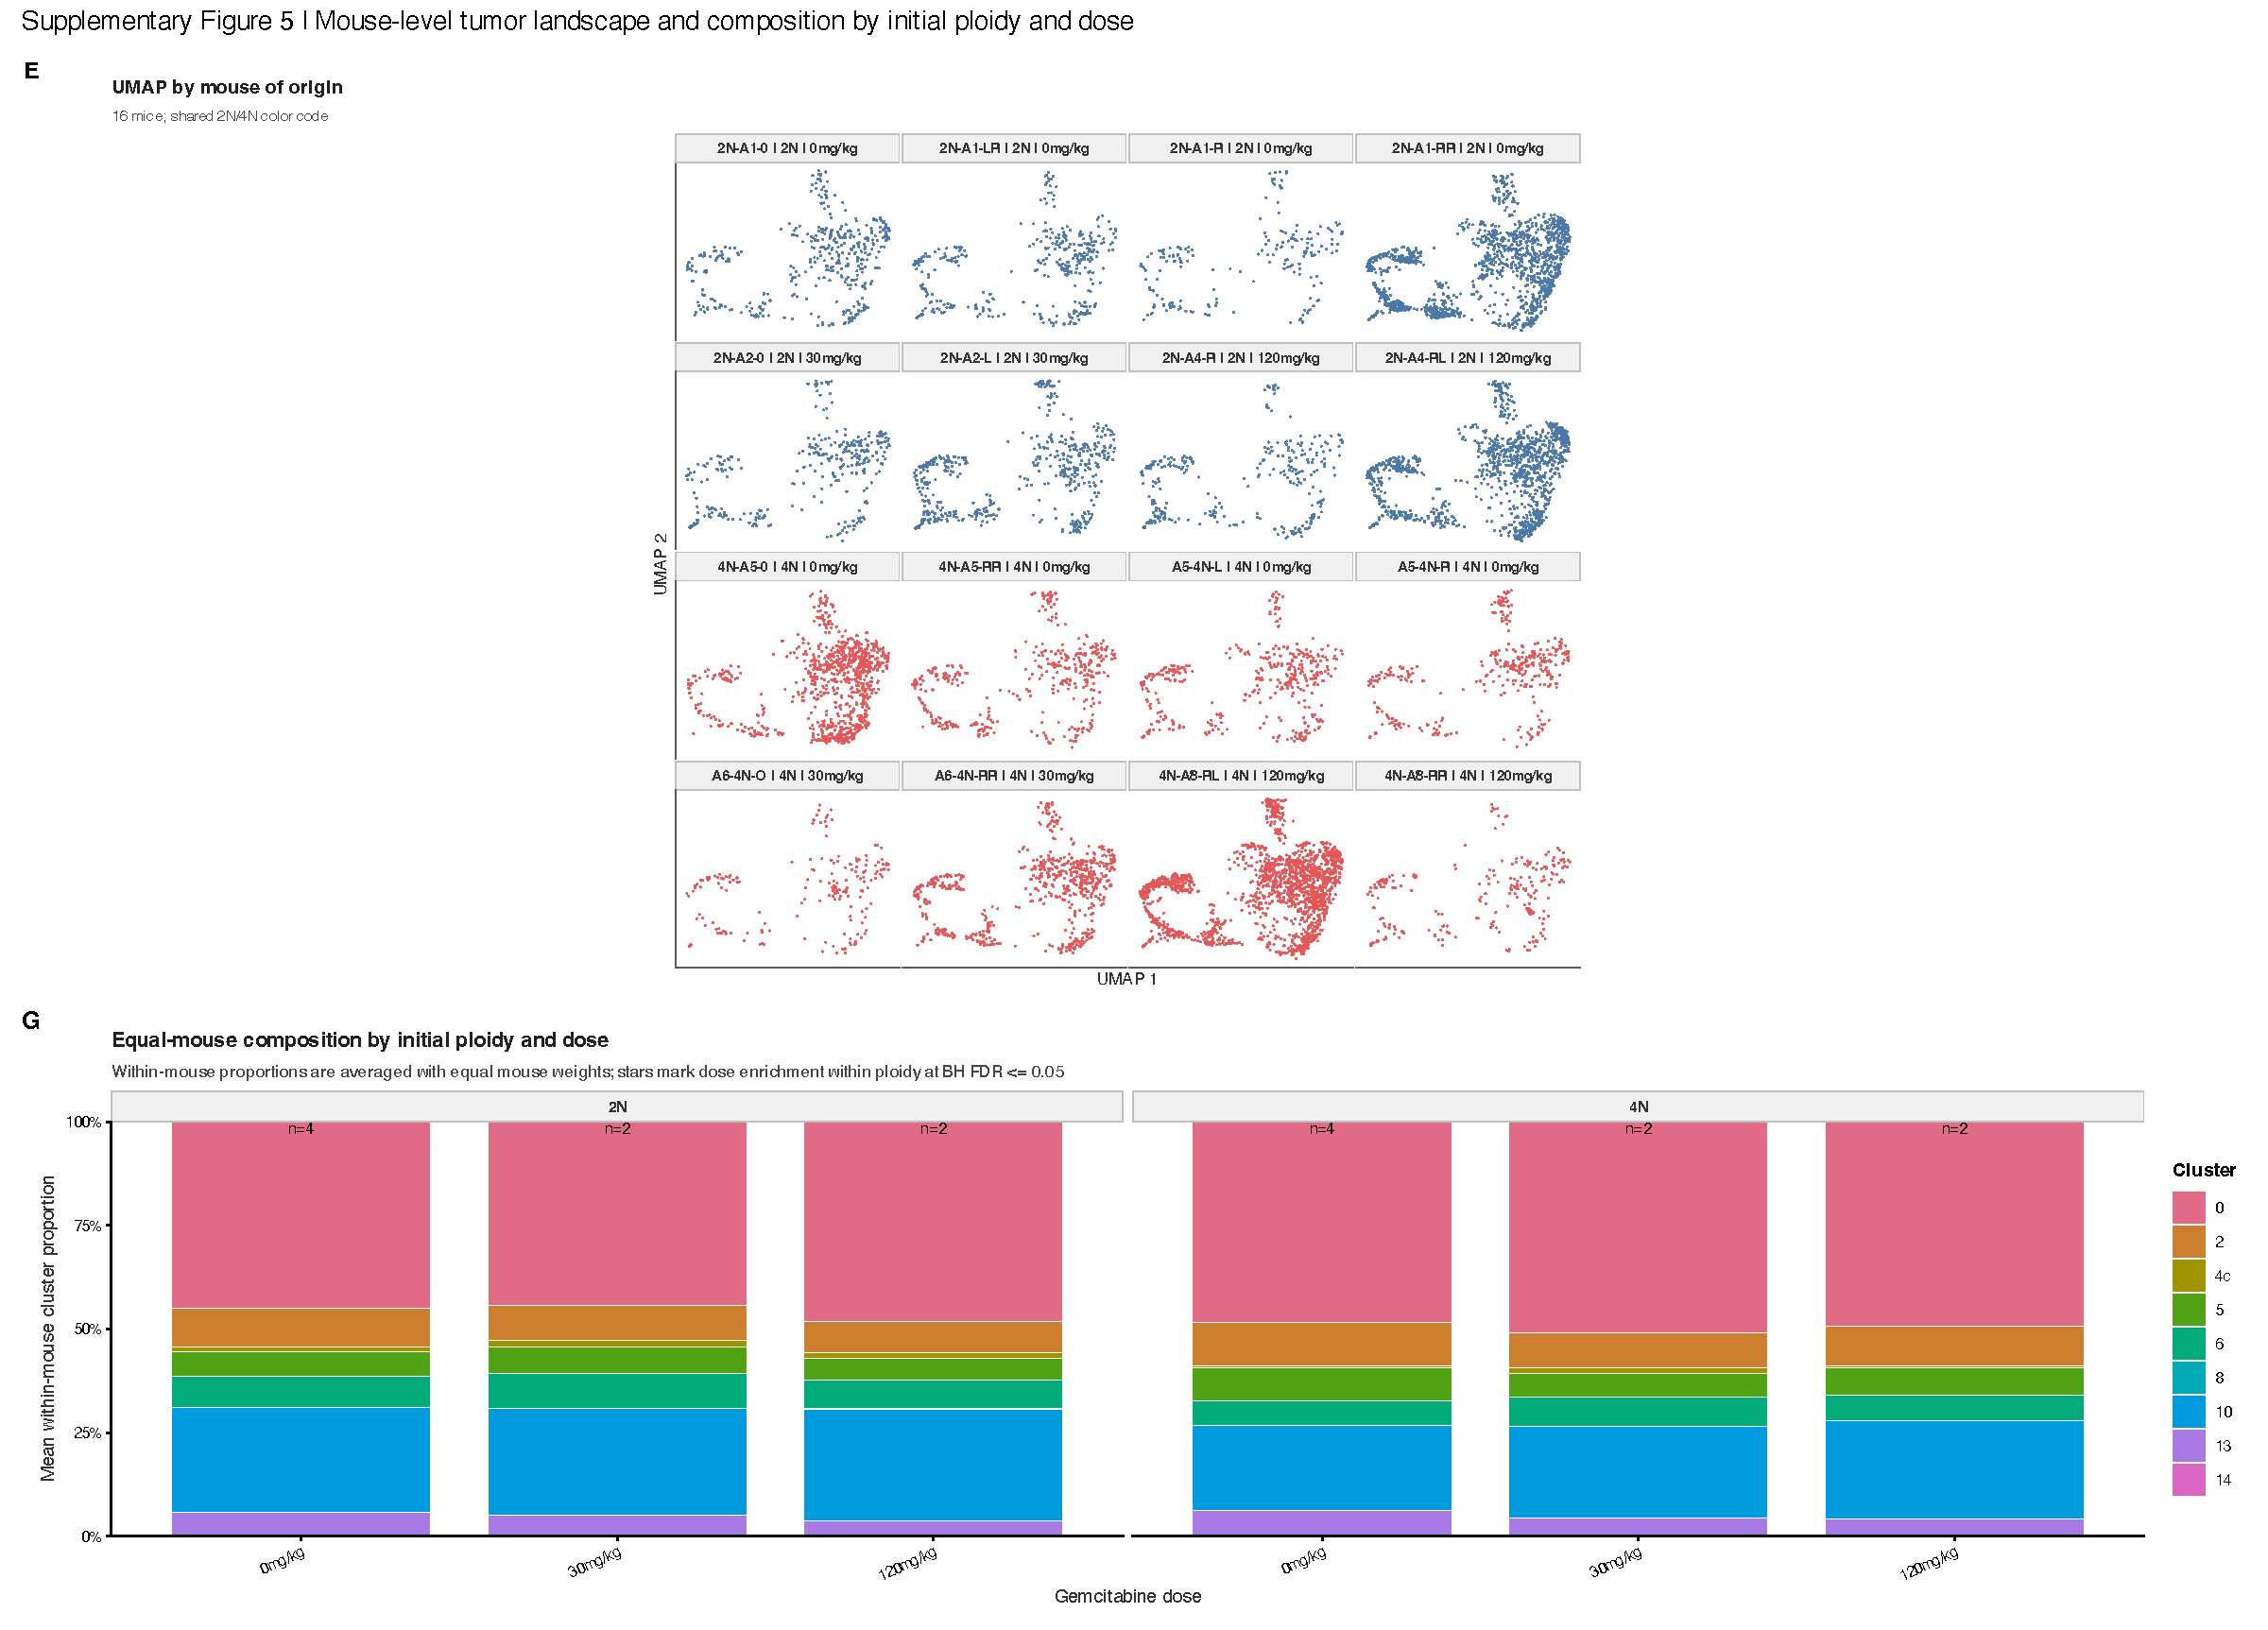
\includegraphics[width=0.95\textwidth,height=0.85\textheight,keepaspectratio]{figures/Supplementary/panel_SuppFig5_composite.pdf}
\caption{\footnotesize
\textbf{Initial ploidy, treatment, and mouse-level composition of xenograft-derived tumor cells.}
\textbf{(A--D)} Tumor-cell UMAPs colored by cluster, initial ploidy, gemcitabine dose, and S-phase score, respectively.
\textbf{(E)} Tumor-cell UMAP faceted by mouse of origin, with initial ploidy and dose shown in each facet label.
\textbf{(F)} Within-mouse cluster proportions; each mouse sums to 100\%. Because each displayed mouse is one biological sample, this panel is descriptive and has no inferential asterisks.
\textbf{(G)} Mean within-mouse cluster proportions by initial ploidy and dose, with equal mouse weights; labels report the number of mice in each group, and asterisks mark positive dose enrichment within initial-ploidy strata at panel-wide BH FDR $\leq 0.05$ using exact mouse-label permutations.
\textbf{(H,I)} Mean within-mouse cluster proportions by gemcitabine dose and initial ploidy, respectively; every mouse contributes equally within its group. Asterisks mark positive enrichment using exact permutations within initial-ploidy strata for H and within dose strata for I, followed by panel-wide BH correction.
}
\label{fig:supp_tumor_composition}
\end{figure}

\clearpage

\begin{figure}[p]
\centering
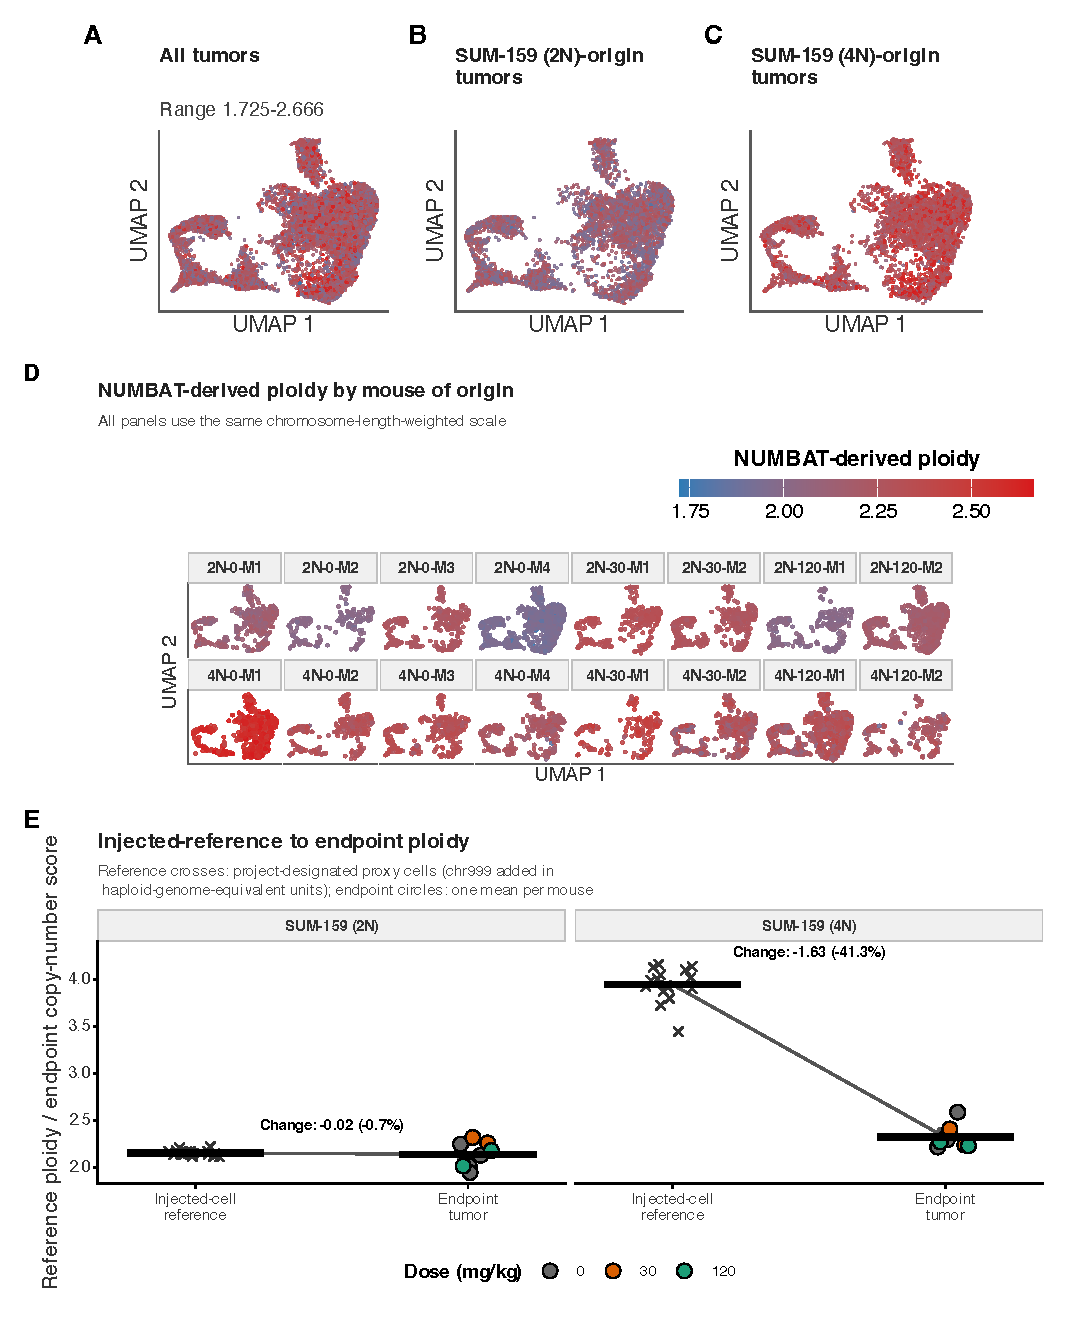
\includegraphics[width=0.80\textwidth,height=0.88\textheight,keepaspectratio]{figures/Supplementary/panel_SuppFig6_composite.pdf}
\caption{\scriptsize
\textbf{Endpoint tumor ploidy and NUMBAT-derived copy-number states across the xenograft-derived cellular landscape.}
\textbf{(A)} Final-QC tumor-cell UMAP colored by NUMBAT-derived chromosome-length-weighted ploidy across all tumors.
\textbf{(B,C)} Ploidy among QC-retained tumors initiated from 2N and 4N cells, respectively, shown on the common scale used in A.
\textbf{(D)} NUMBAT-derived ploidy among the final-QC tumor cells, faceted by mouse of origin.
\textbf{(E)} Cell-by-chromosome heatmap for the exact 9,832 final-QC tumor cells (4,880 2N-origin and 4,952 4N-origin; 5,335 treated) selected from the validated 14,125-cell CBS inventory. Clusters 3, 4, 9, and 9c were excluded. Each entry is the length-weighted mean copy-number state across the segments available for that chromosome within its origin-specific CBS schema; no cross-run locus alignment was performed. Columns follow chromosomes 1--22, and rows are ordered by injected origin, dose, mouse, ploidy, and cell identifier without clustering. Side bars annotate injected origin and mouse; gray denotes an unavailable chromosome-level value.
\textbf{(F)} Project-designated lineage-matched injected-state karyotype proxies (crosses; 20 2N-A7M and 16 4N-A5M metaphases) compared with one final-QC terminal mean per mouse (circles; color indicates dose). These proxy populations are not same-passage measurements of the A6M and A4M inocula. Reference ploidy is the sum of the autosomal chromosome-length-weighted estimate and the chromosome-999 unassigned-DNA value in haploid-genome-equivalent units. Horizontal bars show the proxy-cell mean (2N, 2.151; 4N, 3.947) or the mean of eight endpoint mouse means (2N-origin, 2.136; 4N-origin, 2.319), and arrows show the descriptive proxy-to-endpoint change. The 4N-origin mean was 41.3\% below its reference proxy, and the 2N--4N mean separation contracted by 89.8\%. No formal \(P\) value is attached because each reference represents one culture-level biological unit, the endpoint tumors are independently replicated mice, and the two origin-specific NUMBAT outputs use different schemas and calibration.
}
\label{fig:supp_endpoint_ploidy}
\end{figure}

\clearpage

\begin{figure}[p]
\centering
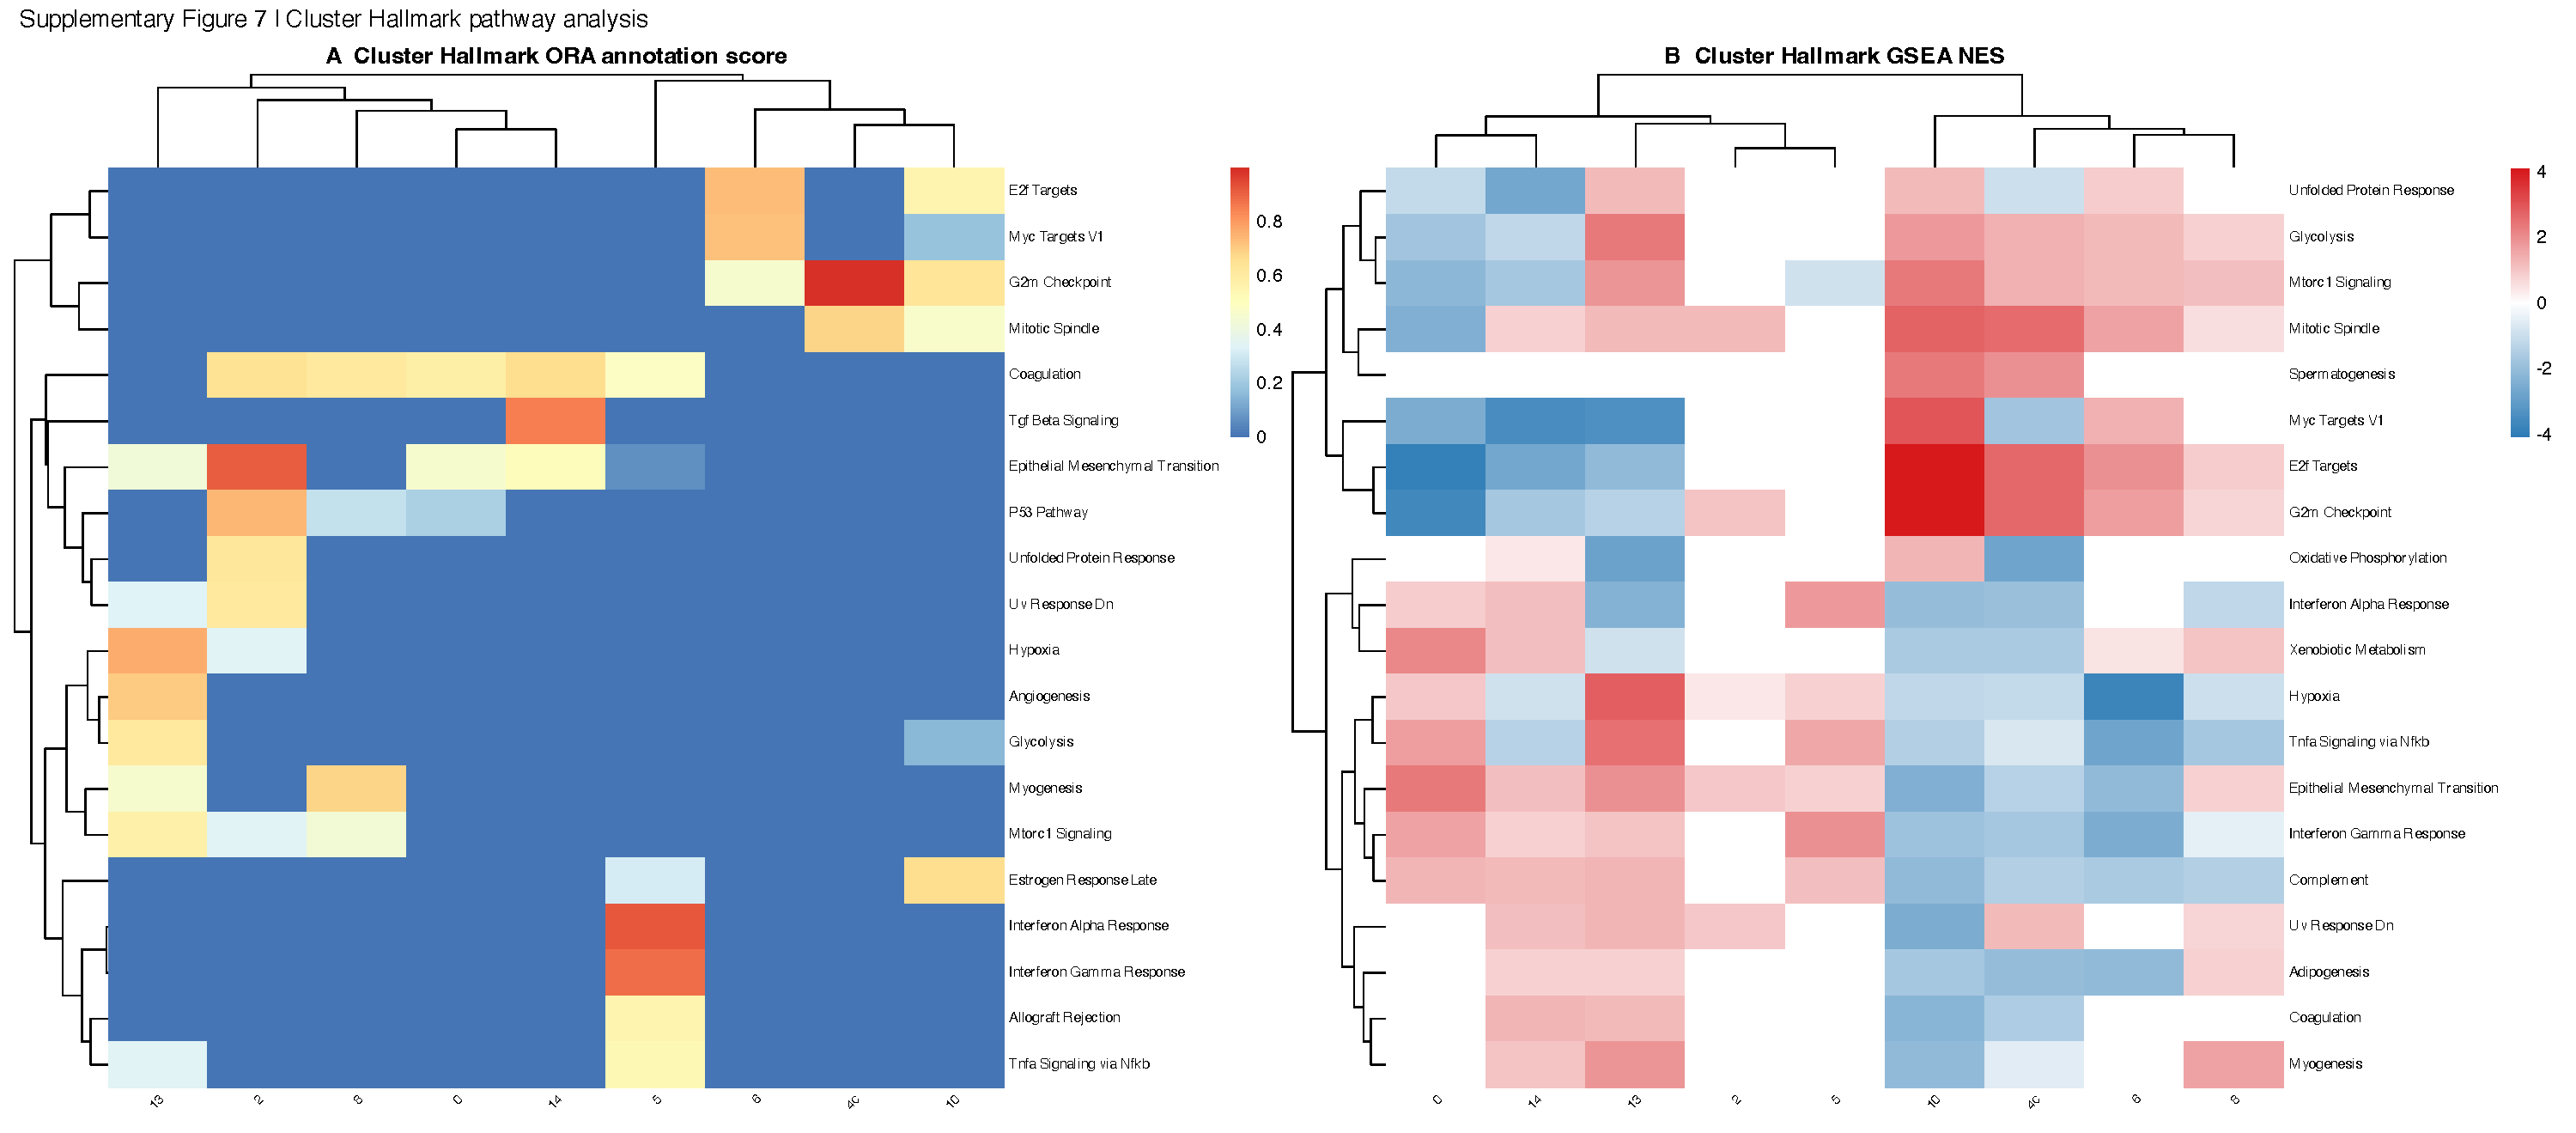
\includegraphics[width=\textwidth,height=0.88\textheight,keepaspectratio]{figures/Supplementary/panel_SuppFig7_composite.pdf}
\caption{\footnotesize
\textbf{Cluster-level Hallmark pathway analysis in xenograft-derived tumor cells.}
\textbf{(A)} Cluster-versus-rest Hallmark over-representation analysis (ORA) annotation scores across the nine clusters.
\textbf{(B)} Cluster-versus-rest Hallmark gene-set enrichment analysis (GSEA) normalized enrichment scores across the same clusters. The reviewed matrices retain exact GRCh38-prefixed RNA features before normalization and differential-expression analysis.
}
\label{fig:supp_cluster_hallmark}
\end{figure}

\clearpage


\begingroup
\renewcommand{\thefigure}{8}
\begin{figure}[p]
\captionsetup{name=Supplementary Figure}
\centering
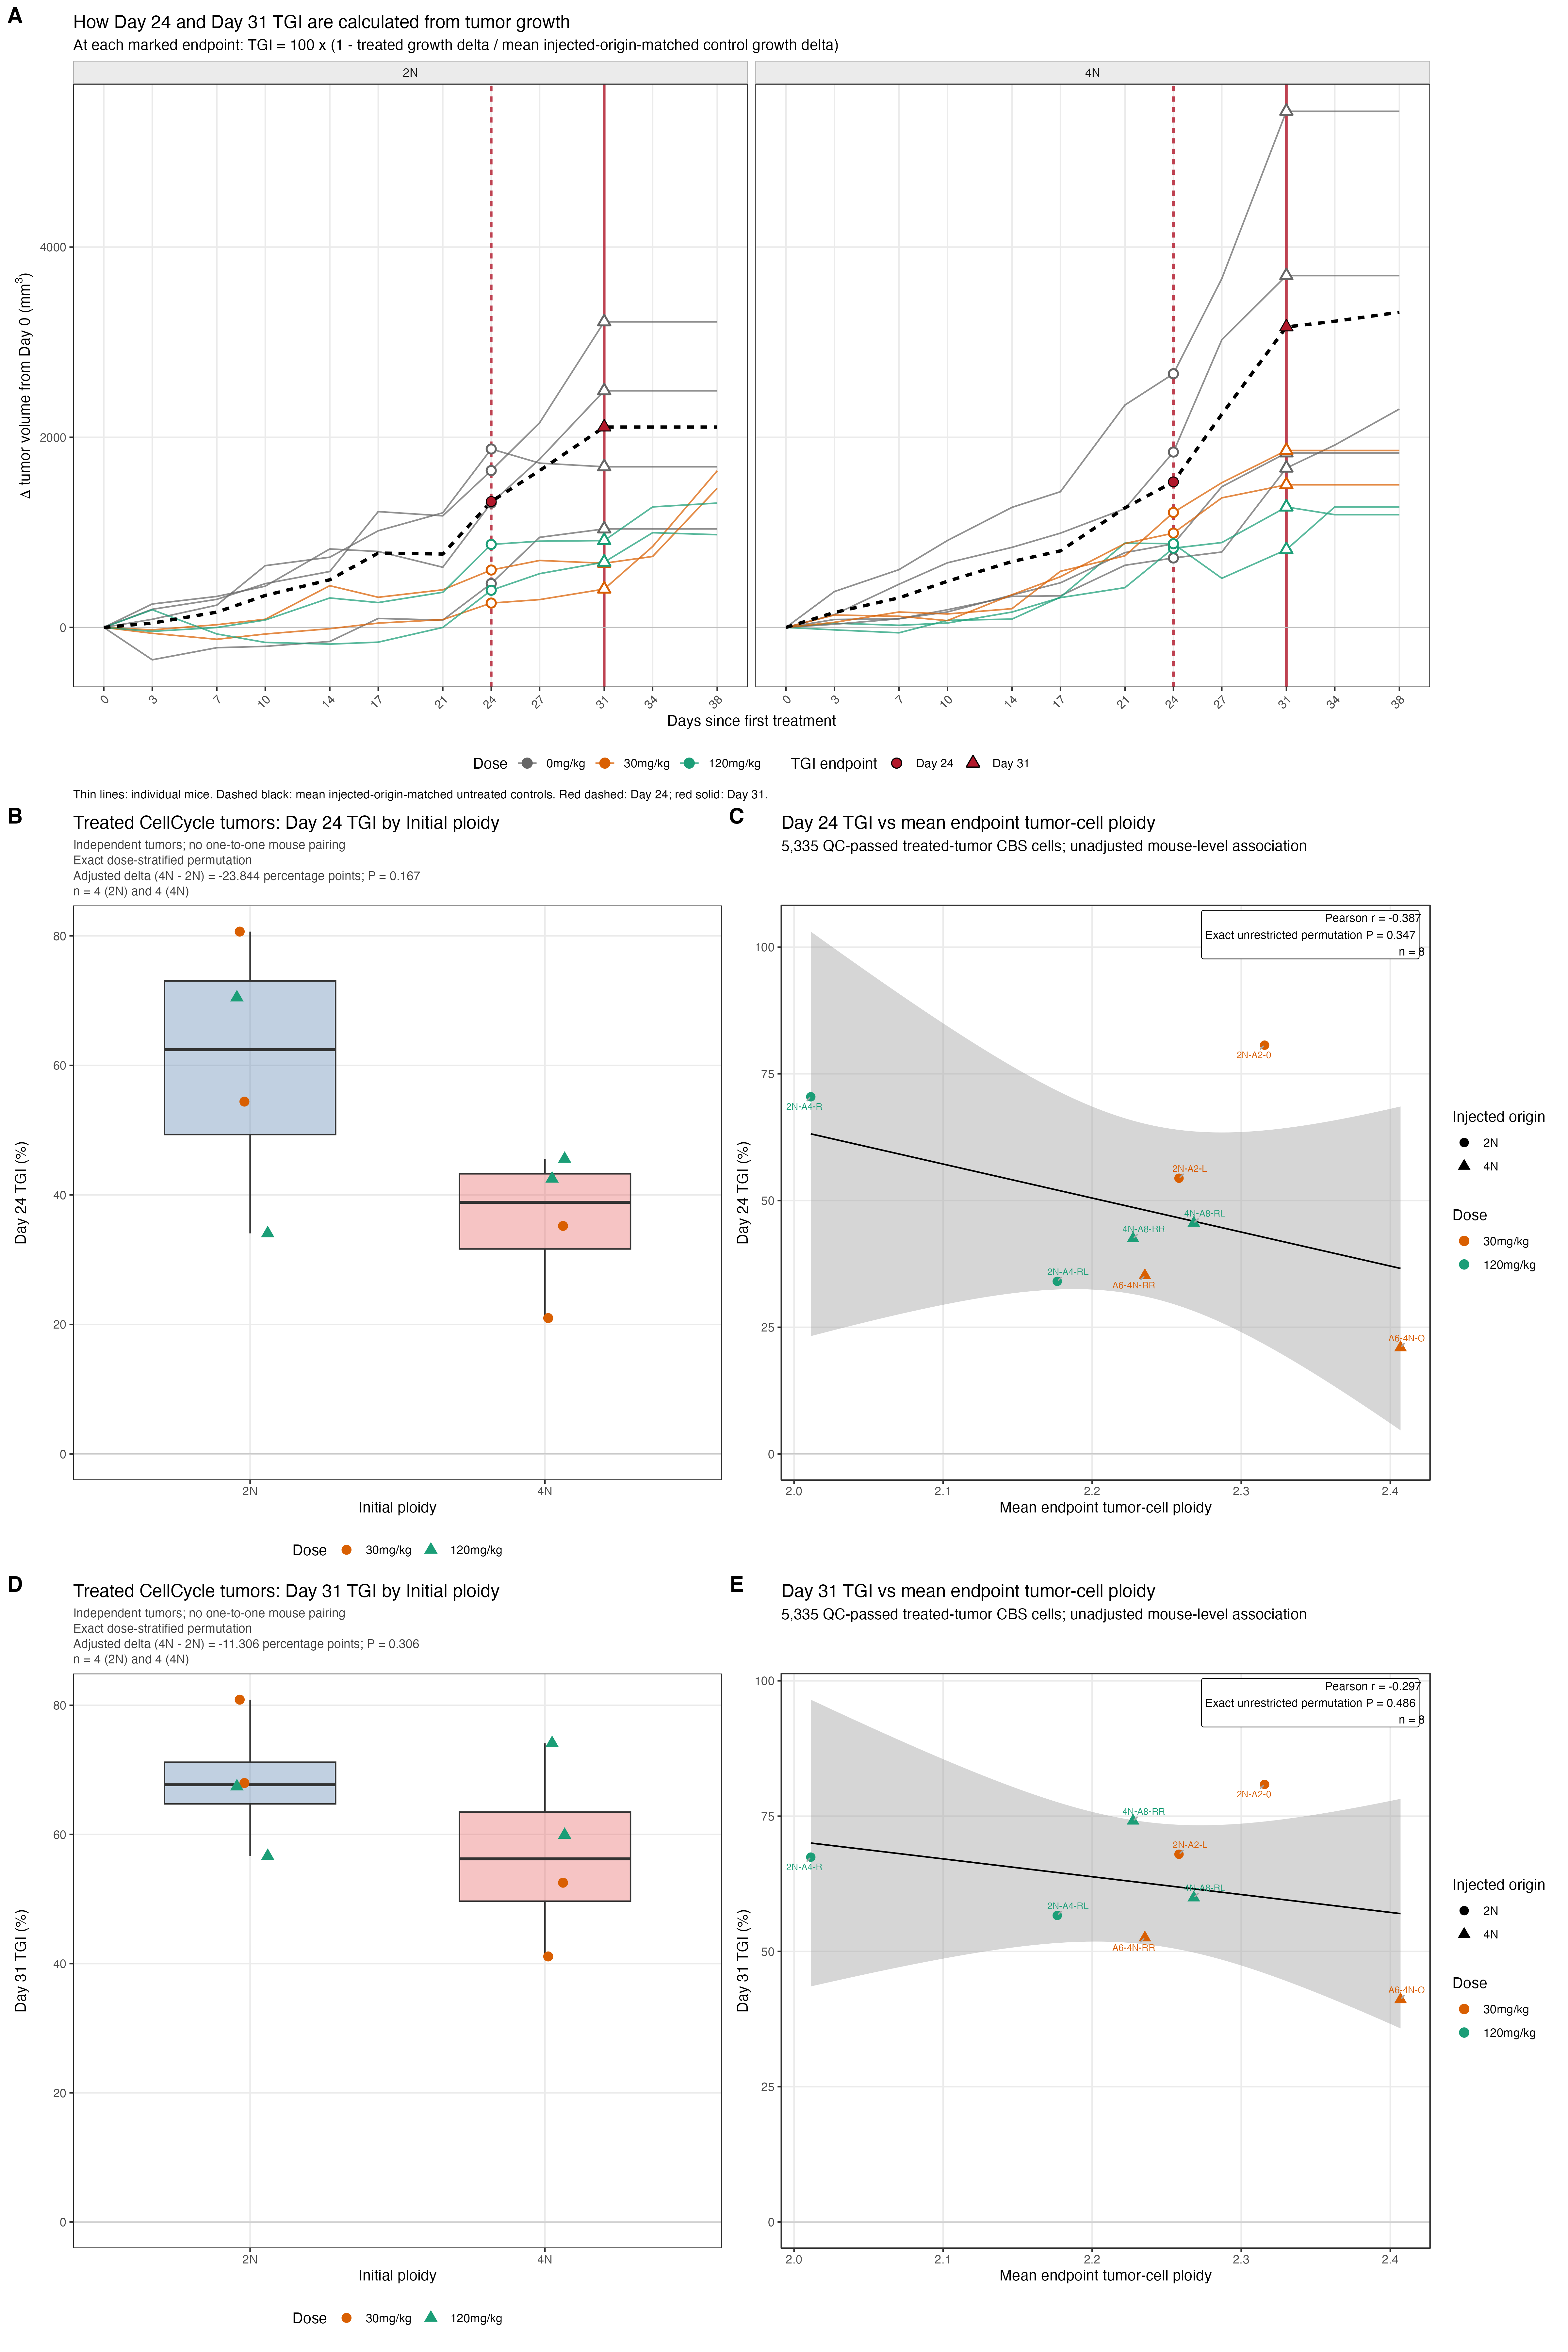
\includegraphics[height=0.68\textheight,keepaspectratio]{figures/Figure7_Supplement/Figure7_Supplement.png}
\caption{\footnotesize
\textbf{Later TGI endpoints preserve the direction but attenuate the magnitude of the injected-origin and endpoint-ploidy associations.}
\textbf{(A)} Baseline-adjusted tumor-growth trajectories for tumors initiated with near-diploid (2N) or near-tetraploid (4N) SUM-159 cells, with Days 24 and 31 marked as alternative TGI endpoints. Thin lines show individual mice and dashed black lines show the mean untreated-control trajectory matched by initial ploidy. At each endpoint, TGI was calculated as \(100\times[1-(\text{treated growth delta}/\text{mean matched-control growth delta})]\).
\textbf{(B)} Day-24 TGI in treated tumors grouped by initial ploidy. The dose-adjusted 4N-minus-2N difference was -23.8 percentage points (exact dose-stratified permutation \(P=0.167\); \(n=4\) tumors per initial-ploidy group).
\textbf{(C)} Unadjusted mouse-level association between Day-24 TGI and mean endpoint tumor-cell ploidy (Pearson \(r=-0.387\), exact unrestricted permutation \(P=0.3469\); \(n=8\)).
\textbf{(D)} Day-31 TGI in treated tumors grouped by initial ploidy. The dose-adjusted 4N-minus-2N difference was -11.3 percentage points (exact dose-stratified permutation \(P=0.306\); \(n=4\) tumors per initial-ploidy group).
\textbf{(E)} The corresponding unadjusted association at Day 31 (Pearson \(r=-0.297\), exact unrestricted permutation \(P=0.4857\); \(n=8\)). In B--E, only treated tumors are included; colors indicate dose, and shapes in C and E indicate injected origin. Lines and 95\% confidence intervals in C and E show the raw mouse-level fits. Panels C and E use the same 5,335-cell QC-retained treated-tumor universe as Fig.~\ref{fig:in_vivo_pseudotime_tgi}K.
}
\label{fig:figure7_tgi_sensitivity}
\end{figure}
\endgroup

\clearpage


\subsection{In-vivo experiments} \label{invivo}

This study utilized near-diploid (2N) and near-tetraploid (4N) variants of the SUM159 triple-negative breast cancer cell line (\texttt{SUM159\_NLS\_2N\_A6M} and \texttt{SUM159\_NLS\_4N\_A4M}, respectively). For the \textit{in vivo} experiments, 1~$\times$~10$^6$ cells were injected orthotopically into mice. A total of 40 mice were used, divided into two main groups based on the injected cell line:
\begin{itemize}
    \item \textbf{2N group:} 20 mice were injected with the near-diploid cell line.
    \item \textbf{4N group:} 20 mice were injected with the near-tetraploid cell line.
\end{itemize}
Within each group, mice were further randomized into four Gemcitabine treatment arms (n=5 mice per arm): 0~mg/kg (vehicle), 30~mg/kg, 60~mg/kg, or 120~mg/kg. Tumors were harvested at specified endpoints.

\subsection{In-vivo derived scRNA-seq analysis}

Single-cell RNA sequencing was performed on 18 lesions: 16 primary tumors and two metastatic lesions. No tumor cells from either metastatic lesion passed quality control, so Figures~\ref{fig:in_vivo_pseudotime_tgi} and Supplementary Figs.~\ref{fig:supp_cellular_landscape}--\ref{fig:supp_cluster_hallmark} analyze the 16 primary tumors.

The two cell lines (\texttt{SUM159\_NLS\_2N\_A6M} and \texttt{SUM159\_NLS\_4N\_A4M}) were also sequenced, yielding a total of 20 scRNA-Seq datasets.


\subsubsection{Single-cell RNA-seq preprocessing and quality control}
The reproducible transcriptomic boundary comprised 18 Cell Ranger \texttt{filtered\_feature\_bc\_matrix.h5} matrices generated against a combined human (GRCh38) and mouse (GRCm39) reference: 16 primary tumors and the two cultured reference populations. The FASTQ-to-Cell-Ranger invocation is not retained in this repository. For each primary tumor, the analysis retained the Cell Ranger barcodes present in the corresponding canonical postprocessed NUMBAT CBS export; consequently, tumor-cell eligibility was inherited from that external upstream copy-number workflow rather than recomputed here by a majority-UMI species classifier. For each cultured reference, cells were required to have at least 200 detected features and 500 UMIs, no more than the sample-specific 99th percentile of either measure, and at most 20\% mitochondrial counts; \texttt{scDblFinder} singlets were then retained. Each sample was independently transformed with Seurat \texttt{SCTransform}, regressing the computed mitochondrial fraction and retaining all genes.

\subsubsection{Copy number analysis}

\paragraph{NUMBAT inference and reproducibility boundary:} Single-cell copy-number states were inferred with NUMBAT in separate 2N-origin and 4N-origin analyses. The reproducible boundary of this repository begins with the checksum-pinned postprocessed cell-by-segment CBS exports. Upstream NUMBAT artifacts may exist outside this repository, but the allele-count inputs, clone posteriors, segment tables, phylogenies, logs, configuration, and executable workflow are not retained and versioned here, and their completeness and exact correspondence to all 16 canonical CBS exports have not been established here. We therefore do not claim that the upstream NUMBAT inference can be independently reproduced from this repository. The origin-specific exports differ in segment schema and calibration; downstream cross-origin analyses treat them as postprocessed CN scores rather than locus-aligned joint inference.

\paragraph{Downstream ploidy analysis:} The validated source inventory comprised 16 exported cell-by-segment CBS matrices, one for each sequenced primary tumor, containing 14,125 cells in total. Downstream figure and association analyses matched this inventory to the exact final QC-curated tumor-cell universe and retained 9,832 cells (4,880 2N-origin and 4,952 4N-origin), including 5,335 treated cells; clusters 3, 4, 9, and 9c were excluded. The project-designated injected-state references were chromosome-level karyotype CBS matrices for the lineage-matched 2N-A7M population (20 metaphases) and 4N-A5M population (16 metaphases). They are proxies rather than same-passage measurements of the A6M and A4M inocula. Matrix filenames, byte sizes, and SHA-256 checksums were frozen in separate terminal and injected-reference manifests. For every terminal cell \(c\), autosomal chromosome-length-weighted ploidy was calculated as
\[
p_c = \frac{\sum_{j\in A_c} L_j C_{cj}}{\sum_{j\in A_c} L_j},
\]
where \(C_{cj}\) is the copy-number value for autosomal segment \(j\), \(L_j\) is its length, and \(A_c\) contains entries with a finite value for that cell. The corresponding coverage fraction was \(\sum_{j\in A_c}L_j/\sum_jL_j\). The canonical 14,125-row source table was regenerated from the 16 matrices by the committed \texttt{weighted\_ploidy.py} implementation and required to match the frozen table byte-for-byte before the 9,832-cell QC selection was applied. For each injected-reference metaphase, the same autosomal length-weighted summary was first calculated across chromosomes 1--22. The chromosome-999 entry, \(u_c\), represents unassigned extra DNA in haploid-genome-equivalent units; the injected proxy was therefore \(p^{\mathrm{proxy}}_c=p^{\mathrm{autosomal}}_c+u_c\). This correction yielded mean 2N and 4N proxies of 2.151 and 3.947, respectively.

For Supplementary Fig.~\ref{fig:supp_endpoint_ploidy}E, segment values for the 9,832 QC-retained cells were reduced separately within each terminal CBS schema to a length-weighted available-segment mean for each chromosome and cell. The resulting 22 chromosome summaries were juxtaposed for display, but loci and segment boundaries were not aligned between the independently inferred 2N-origin and 4N-origin runs. Cells were ordered by injected origin, gemcitabine dose, mouse, ploidy, and cell identifier; chromosomes were ordered 1--22, with no row or column clustering. Mouse and injected-origin annotations were displayed with \texttt{pheatmap}.

For Supplementary Fig.~\ref{fig:supp_endpoint_ploidy}F, the QC-retained terminal cell values were first averaged within mouse so that each of the 16 tumors contributed one observation. Injected-reference metaphases were plotted individually, and each reference-proxy mean was compared descriptively with the equally weighted mean of the eight endpoint mice from the corresponding injected-origin group. We did not attach a formal \(P\) value because each reference was a single culture-level biological unit rather than an independently replicated set of inocula, and the proxy and endpoint values derive from distinct assays and origin-specific postprocessing. Reduction magnitude, reference and endpoint ranges, cell and mouse counts, and whether endpoint values lay below the reference range were exported as figure metadata. These data support a descriptive proxy-to-endpoint comparison but do not identify the timing of ploidy reduction or establish that it caused the TGI difference.

\paragraph{Endpoint tumor-cell ploidy and TGI:} For Fig.~\ref{fig:in_vivo_pseudotime_tgi}K and Supplementary Fig.~\ref{fig:figure7_tgi_sensitivity}C,E, mouse-level endpoint tumor-cell ploidy was calculated as the arithmetic mean of the finite postprocessed cell-ploidy values among the exact final-QC cells assigned to each tumor. The sample-to-CBS mapping was required to match the unique \texttt{growth\_curve\_harvest} identifier, reproduce every selected cell's value from the canonical 14,125-cell source table, and retain exactly 9,832 QC-passed tumor cells, of which 5,335 belonged to the eight gemcitabine-treated tumors. For each TGI endpoint, the raw Pearson correlation between the eight per-mouse mean endpoint ploidies and the eight raw TGI values was reported. Exact two-sided \(P\) values were obtained by unrestricted enumeration of all \(8!=40{,}320\) assignments of the observed TGI values to the eight endpoint-ploidy means. These descriptive associations were not standardized or adjusted for injected origin or dose and therefore do not estimate an origin- or dose-independent ploidy effect.



\clearpage




\subsubsection{Integration, clustering, and dimensionality reduction}
Three thousand integration features were selected across the 18 sample objects. SCT-normalized CCA anchors were identified with Seurat \texttt{FindIntegrationAnchors}, and the samples were combined with \texttt{IntegrateData}. Fifty PCs were calculated from the integrated assay; PCs 1--30 were used to build the shared-nearest-neighbor graph, perform Louvain clustering at resolution 0.6, and calculate the initial UMAP. This produced the 42,884-cell integrated object used for the reviewed cell-cycle annotation and subsequent deterministic cluster curation described below. The final curated object retained 35,513 cells; PCA and UMAP were recalculated after curation using up to 50 PCs and PCs 1--30, respectively. The final nine labels were curated from the initial clustering rather than obtained by a second unsupervised clustering pass.

\subsubsection{Cell-cycle scoring and reviewed cluster curation}
Cell-cycle scores and phases were calculated on the RNA assay of the 42,884-cell integrated object with Seurat \texttt{CellCycleScoring} and \texttt{cc.genes.updated.2019}. Gene symbols were resolved against the combined-reference feature identifiers by removing a \texttt{GRCh}-release prefix and terminal version suffix for matching. A cluster was designated a cell-cycle candidate when at least two of three prespecified criteria were met: (i) its mean S or G2/M score exceeded the across-cluster mean by one standard deviation, (ii) its S- or G2/M-phase fraction exceeded the corresponding across-cluster mean by one standard deviation, or (iii) its mean position was separated by more than one across-cluster standard deviation on at least one of the first 20 PCs whose absolute correlation with S or G2/M score was at least 0.30. This rule identified clusters 6, 10, 11, and 12.

The reviewed legacy curation then split UMAP-local subsets of initial clusters 4 and 9 into labels 4c and 9c by a deterministic nearest-neighbor, convex-hull, and connected-component rule; merged initial clusters 0, 1, and 7 as cluster 0 and clusters 10, 11, and 12 as cluster 10; and excluded clusters 3, 4, 9, and 9c. PCA and UMAP were recalculated after this curation. The final 35,513-cell Tumor/CellLine object contained nine displayed clusters (0, 2, 4c, 5, 6, 8, 10, 13, and 14), comprising 9,832 xenograft-derived tumor cells and 25,681 cultured cells.


\subsubsection{Sample-balanced cluster composition and Hallmark pathway analysis}
For cluster-composition analyses, the independent unit was a tumor-bearing mouse or a cultured CellLine sample. Cell counts were first converted to within-sample cluster proportions, and samples were then averaged with equal weight within each displayed group so that sequencing depth did not determine a sample's contribution. Positive enrichment was tested on these independent-sample proportions with an exact one-sided, one-group-versus-rest label-permutation test within prespecified exchangeability strata. Context enrichment in Fig.~\ref{fig:in_vivo_pseudotime_tgi}F and Supplementary Fig.~\ref{fig:supp_cellular_landscape}E was tested within injected-ploidy strata; initial-ploidy enrichment in Supplementary Fig.~\ref{fig:supp_cellular_landscape}G was tested within Tumor/CellLine context; dose enrichment in Supplementary Fig.~\ref{fig:supp_tumor_composition}G,H was tested within injected-ploidy strata; and initial-ploidy enrichment in Supplementary Fig.~\ref{fig:supp_tumor_composition}I was tested within dose strata. Benjamini--Hochberg correction was applied across all group-by-cluster contrasts in each panel, and asterisks mark only positive enrichments with FDR $\leq 0.05$. Supplementary Fig.~\ref{fig:supp_tumor_composition}F contains one biological sample per displayed mouse and was therefore treated as descriptive, without inferential stars.

For the cluster-versus-rest Hallmark analyses in Fig.~\ref{fig:in_vivo_pseudotime_tgi}G and Supplementary Fig.~\ref{fig:supp_cluster_hallmark}, exact \texttt{GRCh38-}-prefixed RNA count features were retained, exact \texttt{GRCm39-}-prefixed features were excluded, and unclassified prefixes were rejected before normalization or differential expression. A new human-only RNA object was normalized with Seurat \texttt{LogNormalize} (scale factor 10,000); the mixed-species normalized data layer was not reused. Each of the nine clusters was compared with all remaining cells using Seurat \texttt{FindMarkers} on the normalized RNA data. For over-representation analysis (ORA), upregulated genes were required to have Seurat-adjusted $P<0.05$, log fold change $\geq 0.25$, and an absolute between-group detection-fraction difference $\geq 0.05$; after case-sensitive symbol resolution and deduplication, the top 100 genes by fold change were tested by a one-sided hypergeometric test against Homo sapiens MSigDB 2026.1.Hs Hallmark sets of 15--500 genes, requiring at least three overlapping genes and applying Benjamini--Hochberg correction within cluster. The displayed ORA annotation score is the mean of min--max-scaled overlap, expression, and detection components. For gene-set enrichment analysis (GSEA), genes were ranked by signed $-\log_{10}$ adjusted $P$ value, with fold change used to resolve ranking ties, and duplicate symbols were resolved case-sensitively. \texttt{fgseaMultilevel} was run against the same Hallmark sets (15--500 genes; \texttt{nPermSimple}=10,000; $\epsilon=0$). The ORA and GSEA heatmaps display the 20 pathways with the largest cross-cluster annotation score or absolute normalized enrichment score, respectively; hierarchical clustering of rows and columns changes display order only.

\subsubsection{RNA velocity, CellCycle pseudotime, and tumor-level distribution tests}
Spliced and unspliced counts from the velocyto loom files were matched one-to-one to cells in the final Seurat object. scVelo filtering and normalization used a minimum of 20 shared counts and 2,000 highly variable genes. Moments were calculated on the 30-component Seurat PCA representation with 30 nearest neighbors, velocities were estimated in stochastic mode, and the velocity graph was converted to a 0--1 velocity-pseudotime coordinate rooted in cluster 6. The downstream CellCycle analysis was restricted to the 2,881 xenograft-derived cells in clusters 4c, 6, and 10.

For each mouse, an empirical cumulative distribution function (ECDF) was evaluated on a common 501-point pseudotime grid. Group curves were arithmetic means of the mouse-specific ECDFs, giving every mouse equal weight. Untreated-versus-treated differences were summarized by the root-mean-square difference between group ECDFs, and exact $P$ values were obtained by enumerating all treatment-label assignments that preserved the observed group sizes, both across all 16 tumors and separately within each injected-origin stratum. For Fig.~\ref{fig:in_vivo_pseudotime_tgi}J, each treated tumor's displacement was the ECDF RMSE from the equal-mouse untreated reference matched by injected ploidy origin. Displacement and Day-17 TGI were each centered within dose, their Pearson correlation was reported, and its exact two-sided $P$ value was obtained from all 576 TGI-label permutations within dose. Day-17 TGI was calculated from change since treatment baseline relative to the mean change of the four untreated tumors matched by injected origin. The dose-adjusted injected-origin contrast was estimated with dose as a categorical covariate and tested by exact injected-origin-label enumeration within dose; the same procedure was used for the Day-24 and Day-31 sensitivity endpoints.

\subsubsection{Mouse-aware pseudotime-state expression and pathway analysis}
For Fig.~\ref{fig:in_vivo_pseudotime_tgi}I, exact \texttt{GRCh38-}-prefixed RNA counts from the CellCycle subset were retained before expression filtering, symbol resolution, model fitting, and Homo sapiens pathway analysis; \texttt{GRCm39-}-prefixed and unclassified features were excluded. Pseudotime was divided into 20 equal-width bins, raw counts were summed within each mouse-by-bin combination, and bins containing fewer than five cells were excluded. Genes were retained when CPM exceeded 1 in at least 14 retained sample-bin observations. Pseudobulk libraries were TMM-normalized and analyzed with limma--voom using a five-degree-of-freedom natural spline for pseudotime, categorical gemcitabine dose and injected ploidy origin as nuisance terms, and mouse as the blocking factor in \texttt{duplicateCorrelation}; robust empirical-Bayes moderation was used. No treatment-by-pseudotime interaction was fitted. The prespecified contrast compared mean fitted expression in the accumulated interval [0.30,0.49] with the average of the equally wide left [0.11,0.30) and right (0.49,0.68] neighboring intervals.

Genes were ranked by the moderated $t$ statistic for this contrast and analyzed with \texttt{fgseaMultilevel} against Homo sapiens MSigDB 2026.1.Hs Hallmark, Reactome, and Gene Ontology Biological Process collections (gene-set size 15--500). Unresolved pathways were retried at prespecified \texttt{nPermSimple} budgets of 10,000, 100,000, and 1,000,000; Benjamini--Hochberg adjustment was recomputed across each complete collection. The figure displays up to four positive and four negative pathways per collection among pathways with collection-wide FDR $\leq 0.05$, without backfilling nonsignificant pathways. For visualization, fitted expression was standardized across pseudotime within each leading-edge gene and then averaged across the pathway's leading-edge genes. Enrichment direction describes the accumulated interval relative to its neighboring states and is not a treatment effect at fixed pseudotime.



\clearpage
\bibliography{references_Zotero_VT} 
\bibliographystyle{unsrt}

\end{document}
